% Préambule
\documentclass[a4paper, 12pt, twoside]{book}

% Paquets obligatoires
\usepackage{lmodern}
\usepackage[english, french]{babel}
\usepackage[utf8]{inputenc}
\usepackage[T1]{fontenc}
\usepackage[pdfusetitle, pdfsubject={Mémoire TNAH Florian Langelé 2023}]{hyperref}
    \hypersetup{colorlinks=true, linkcolor=black, urlcolor=blue, citecolor=black}

% Configuration de la mise en page
\usepackage[margin=2.5cm]{geometry}  % Marges du document
\usepackage{parskip}  % Espacement entre les paragraphes
    \parskip=6pt
\usepackage{setspace}  % Mise en forme des paragraphes
    \onehalfspacing
    \setlength\parindent{1cm}

% Configuration de la bibliographie
\usepackage[backend=biber, sorting=nyt, style=enc]{biblatex}
\usepackage[autostyle]{csquotes}
\addbibresource{Ma bibliothèque.bib}
\nocite{*}

% Paquets additionnels
\usepackage{xcolor}  % Gestion des couleurs
\usepackage{animate}
\usepackage{bookmark}
\usepackage{pdfpages}
\usepackage{graphicx}  % Gestion des images
\usepackage{fancyhdr}  % Gestion de l'en-tête et du pied de page
    \pagestyle{headings}
    \pagestyle{fancy}
    \fancyhf{}
    \fancyhead[LE,RO]{\thepage}
    \fancyhead[LO,RE]{\leftmark}
    \setlength{\headheight}{15.5pt}
    \setcounter{secnumdepth}{3}
    \setcounter{tocdepth}{3}
\usepackage{emptypage}  % Gestion des pages vierges
\usepackage{pdfpages}  % Gestion des PDF
\usepackage{shorttoc}  % Gestion du sommaire
\usepackage{caption}
\usepackage{array,multirow,makecell}  % Gestion des tableaux
    \setcellgapes{1pt}
    \makegapedcells
    \newcolumntype{R}[1]{>{\raggedleft\arraybackslash }b{#1}}
    \newcolumntype{L}[1]{>{\raggedright\arraybackslash }b{#1}}
    \newcolumntype{C}[1]{>{\centering\arraybackslash }b{#1}}
\usepackage{minted}  % Gestion du code
    \usemintedstyle{perldoc}

\title{Production et exploitation d’un graphe de connaissances décrivant des archives médiévales: le cas du projet ORESM}
\author{Florian Langelé}

\begin{document}
    \begin{titlepage}
		\begin{center}
			
			\bigskip
			
			\begin{large}				
				ÉCOLE NATIONALE DES CHARTES\\
				UNIVERSITÉ PARIS, SCIENCES \& LETTRES
			\end{large}
			\begin{center}\rule{2cm}{0.02cm}\end{center}
			
			\bigskip
			\bigskip
			\bigskip
			
			\begin{Large}
				\textbf{Florian Langelé}\\
			\end{Large}
			\bigskip
			\bigskip
			\bigskip
                \bigskip
               \bigskip
			
			\begin{Huge}
				\textbf{Production et exploitation d’un graphe de connaissances décrivant des archives médiévales : Le cas du projet ORESM}\\
			\end{Huge}
			\bigskip
			
			\bigskip
			\bigskip
			\bigskip

   
			\vfill
			
			\begin{large}
				Mémoire 
				pour le diplôme de master \\
				\og{} Technologies numériques appliquées à l'histoire \fg{} \\
				\bigskip
				2023
			\end{large}
		\end{center}
	\end{titlepage}

    \thispagestyle{empty}
\cleardoublepage
    
\frontmatter
\chapter{Remerciements}
Avant de débuter ce mémoire je souhaite remercier l'ensemble des personnes qui m'ont permis d'achever cette formation de Master dans de bonnes conditions. 
\par
Mes remerciements vont à mes camarades et le corps enseignant de l'École nationale des chartes, qui m'a fourni un accompagnement idéal. Aux personnels de la BIS pour l'accueil chaleureux auquel j'ai eu droit. A l'équipe du projet ORESM, qui m'a accepté en son sein pour ce stage de quatre mois, et m'a permis de l'achever malgré une longue interruption de deux mois.  Mes remerciements vont en particulier à Florence Clavaud qui a eu de nombreux rôles à mon égard, avec laquelle j'ai eu un plaisir de travailler et surtout beaucoup appris. 
\par 
Évidemment je remercie ma famille pour sa présence à mes côtés et son soutien durant le stage et durant la rédaction de ce mémoire. Enfin je souhaite conclure ces remerciements en aillant un mot pour Laura Chevalier, sans qui je ne serais pas là aujourd'hui et qui m'apporte chaque jour, présent et futur, beaucoup de joie.
\printbibliography
\addcontentsline{toc}{chapter}{Bibliographie}
\chapter{Résumé}
\medskip
Ce mémoire a été rédigé à la suite d'un stage de quatre mois, dans le cadre du Master Technologies numériques appliquées à l’histoire de l’École nationale des chartes. Ce stage a été réalisé au sein du SERVAL (Service de la Valorisation numérique des collections et du soutien à la Recherche) sur le projet ORESM
(Œuvres et Référentiels des Étudiants, Suppôts et Maîtres). Le présent mémoire vise à exposer les réflexions et réalisations qu'ont entraînées le stage. Particulièrement en décrivant la production de métadonnées relatives à des archives médiévales et leurs sémantisations avec l'ontologie RiC-O. Le tout dans le cadre d'un projet de recherche ambitieux.

\bigskip
\textbf{Mots-clés }: Université de Paris; archives; RiC-O; Sparnatural ; graphe de connaissance ; web sémantique ; XSLT; RDF.

\bigskip
\textbf{Informations bibliographiques} : Florian Langelé, \textit{Production et exploitation d’un graphe de connaissances décrivant des archives médiévales : le cas du projet ORESM}, mémoire de master \og  Technologies numériques appliquées à l’histoire \fg  , dir. Florence Clavaud, École nationale des chartes, 2023.
\chapter{Introduction}
Un projet de recherche passe nécessairement par de nombreuses étapes. De sa conception à sa réalisation, de l'idée qui germe de l'esprit à la dernière pierre posée il y aura toujours une multitude d'échanges, d'échecs, de remises en question et de réussites pour arriver finalement au résultat voulu. D'autant plus quand le projet innove sur un ou plusieurs aspects de son champ d'action. C'est le cas du projet ORESM conduit par la Bibliothèque Interuniversitaire de la Sorbonne (BIS).
\par
Dans ce mémoire nous présenterons les réflexions, décisions et réalisations qui ont eu lieu au cours du stage de quatre mois au sein du projet ORESM. Ce mémoire pourra permettre de guider la réflexion concernant le traitement et l'exploitation de données relatives à des archives médiévales. Il dresse une feuille de route rétrospective de la production à l'exploitation de ces données en s'appuyant sur l'expérience acquise durant le stage tout en englobant le propos dans le contexte du projet ORESM qui a ses enjeux bien particuliers. Pour résumer nous nous attacherons à expliquer comment les métadonnées archivistiques médiévales de forte granularité du projet ORESM ont été sémantisées afin d'être rendues exploitables par des chercheurs et étudiants.
\par
Nous débuterons ce mémoire par une partie présentant le contexte de notre stage : le projet ORESM, ses différents enjeux et l'avancement de celui-ci avec une présentation des différentes réalisations avant le début du stage. Suivra une partie qui présentera les données issues des dépouillements d'archives réalisés avant notre stage, le processus de sémantisation de ces données, tout en s'attachant à présenter les avantages et inconvénients du modèle suivi. En troisième partie, nous présenterons les premières utilisations que nous avons pu faire des données sémantisées : import dans une base de graphes, ébauche d'une interface de requête sur les données. Enfin, avant de conclure nous ferons un bref bilan du stage tout en présentant quelques pistes pour la poursuite du projet ORESM. Puisque le GitHub de travail du projet ORESM est privé, un \href{https://github.com/Florian-Langele/Memoire-de-stage-TNAH}{GitHub} a été créé pour stocker les livrables du stage associés à ce mémoire.
\mainmatter
\part{Contexte d'un projet ambitieux aux multiples enjeux et facettes}
\chapter{Présentation d'ORESM}
\og \textit{Nous devons espérer (...) que l'autorité publique prendra quelque jour les mesures nécessaires pour concentrer définitivement, du moins autant que possible, ces documents, qui perdent par leur dispersion une grande partie de leur valeur, et pour mettre fin à un état des choses aussi contraire à la loi qu'à l'intérêt des lettres.}\fg  Auguste Vallet de Virville\footnote{Archiviste et historien français né en 1815 et mort en 1868.}, \textit{Histoire de l'instruction publique en Europe et principalement en France, depuis le christianisme jusqu'à nos jours}, 1849.
\section{Origine}
On ne peut pas dissocier le projet ORESM (Œuvres et Référentiels des étudiants, Suppôts et Maîtres) de \textit{Studium Parisiense}\footnote{\href{http://studium.univ-paris1.fr/}{http://studium.univ-paris1.fr/}} qui est une base de données prosopo-bio-bibliographique. Initialement débuté comme un projet pédagogique dans les années 1970, il enseignait aux élèves la construction d'une base de données à partir de leurs propres dépouillements de répertoires biographiques. Au fil des années la masse des données s'est alourdie pour arriver à près de 20 000 fiches. C'est en 2019, quand Jean-Philippe Genet\footnote{Médiéviste spécialiste de l’Angleterre et professeur émérite d’histoire médiévale à la Sorbonne.} initie la restructuration de la base de données \textit{Studium Parisiense}, que débute la réflexion qui débouchera au projet ORESM. Il émet la volonté de valoriser son gisement de données en rendant ces données consultables et utilisables. Pour réfléchir aux différents moyens et formes qui peuvent être mis en œuvre, la BIS recrute pour un stage de quatre mois Lucie Vieillon étudiante du master \og\textit{Technologiques numériques appliquées à l'histoire}\fg. Au cours de cette période elle va participer à la rédaction d'un dossier de demande de financement dans le cadre de l'appel à projets Collex Persée, qui conduira à une première définition des objectifs du projet ORESM. Il est alors proposé de mettre en valeur les données prosopographiques venant de \textit{Studium Parisiense} et les données patrimoniales issues des archives de l'université sur un unique portail web. On permettrait ainsi aux chercheurs de bénéficier d'un unique point d'accès pour se retrouver dans le contenu des différentes institutions possédant des archives de l'université. 
\par
La dispersion des archives relatives à l'université de Paris n'est pas récente. En effet à la Révolution française il y a une volonté de regrouper les fonds d'archives du clergé aux Archives nationales,  suivant la loi du 7 messidor de l'an II. Cette volonté est exécutée de manière partielle se concentrant principalement sur les archives domaniales et laissant éparpillées un grand nombre d'archives relatives à l'université dans différentes institutions comme le collège Louis-le-Grand, l'Hôtel de ville, la bibliothèques Mazarine etc. L'envie de regrouper les archives de l'ancienne université va émerger au cours du siècle suivant. En 1837, Auguste Vallet de Viriville a été chargé par François Guizot\footnote{Homme d'état français. Né en 1787 et mort en 1874, il est important dans l'histoire de l'éducation en France, principalement pour la loi de 1833 qui porte son nom, qui impose à chaque commune de plus de 500 habitants d'avoir une école primaire.} de mettre en ordre les archives de l'ancienne université de Paris. Il a intégré dans le fonds des registres qui étaient restés en possession de la bibliothèque de la Sorbonne. Au fur et à mesure des regroupements successifs du \textsc{XIX}\ieme{} siècle le nombre d'institutions en possession d'archives relatives à l'université de Paris se réduit pour n'être finalement de nos jours plus que la BIS et les Archives nationales, en majorité, ainsi que la Bibliothèque interuniversitaire de Santé (BIUS).
\par
\begin{figure}[!h]
    \centering
    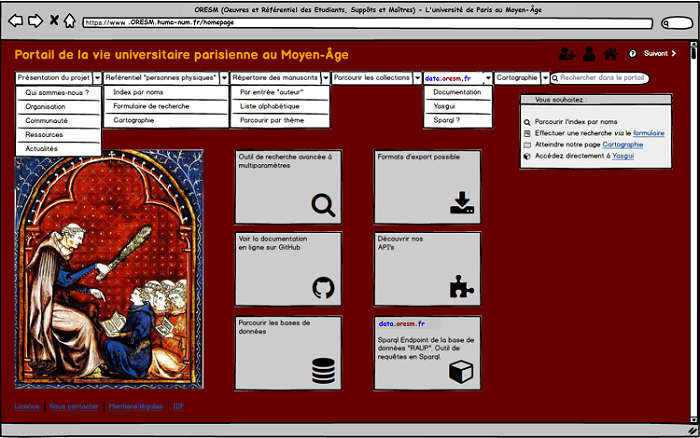
\includegraphics[width=1\linewidth]{images/oresm origine.png}
    \caption{Maquette présentant l'idée initiale du portail ORESM.}
    \label{fig:oresm-origine}
\end{figure}
Finalement il avait été décidé que le projet ORESM se composerait de plusieurs réalisations accessibles par le portail web centralisateur. Un inventaire virtuel regroupant les différentes notices des archives concernant l'université sur la période étudiée, un référentiel des personnes liées à celle-ci, un répertoire des manuscrits, les données contenues dans ces trois composants étant par ailleurs agrégées ou rendues accessibles via une base de données. Plus récemment le projet ORESM a prévu d'ajouter une corde d'édition numérique à son arc avec le projet ECRU (éditions critiques relatives à l’Université de Paris), annexe du projet ORESM, qui vise à encoder des éditions critiques d'actes à l'aide de l'IA\footnote{\og Intelligence Artificielle\fg  Ensemble de théories et de techniques mises en œuvre en vue de réaliser des machines capables de simuler l'intelligence humaine.}. L'encodage se fera en XML-TEI. L'innovation de cette approche réside dans le corpus qui est en latin, aucun autre projet n'avait utilisé l'IA pour réaliser un balisage automatique sur du texte en latin. Les éditions sont tirées des grands ouvrages relatifs aux archives de l'université de Paris en commençant par le \og \textit{Chartularium Universitatis Parisiensis}\fg d’Heinrich Denifle et Emile Châtelain. Le projet ECRU est à ses débuts mais il enrichira à terme les référentiels et la base de données d'ORESM notamment concernant les entités nommées.
\section{Les acteurs}
\subsection{La BIS}
La BIS porte le projet à partir de son service le SERVAL (Service de la Valorisation numérique des collections et du soutien à la Recherche). Son nom est assez explicite concernant sa vocation. Avec les outils numériques disponibles le SERVAL va réaliser des projets de valorisation de sources historiques touchant de près ou de loin à la vie universitaire parisienne. Comme autres projets actuellement portés nous pouvons citer \og ès lettres\fg\footnote{\href{https://www.collexpersee.eu/projet/es-lettres/}{https://www.collexpersee.eu/projet/es-lettres/}} qui porte sur la numérisation et la valorisation des thèses françaises du \textsc{XIX}\ieme{} siècle avec une exposition virtuelle\footnote{\href{https://nubis.univ-paris1.fr/s/theses-doctorats-es-lettres-19-siecle-exposition-devenir-savant/page/introduction}{Lien vers cette exposition virtuelle}}, et une base de données. Nous pouvons également citer le projet PRET19 \footnote{Projet de Répertoire des Emprunteurs et Titres empruntés au \textsc{XIX}\ieme{} siècle à l’université \href{https://www.collexpersee.eu/projet/pret19/}{https://www.collexpersee.eu/projet/pret19/}} qui numérise les registres de prêt de plusieurs bibliothèques parisiennes en commençant au \textsc{XIX}\ieme{} siècle. En plus de cette numérisation le projet prévoit d'utiliser un OCR\footnote{\og Optical Character Recognition\fg  Procédé qui consiste à extraire automatiquement le texte d'une image numérique.} pour extraire des données des registres et construire une base de données accessible en ligne. Ces projets illustrent clairement la mission du SERVAL c'est à dire la production d'outils numériques qui serviront à alimenter la recherche sur des thèmes relatifs à l'histoire de l'université de Paris. Le projet ORESM à la BIS est actuellement dirigé par Laurence Bobis, directrice de la bibliothèque. L'équipe travaillant sur le projet est composée de Laurie Aoustet, adjointe de la cheffe du SERVAL, Arsène Georges et Sébastien Clément.
\subsection{Le LaMOP}
Le Laboratoire de Médiévistique Occidentale de Paris est co-porteur du projet. Crée en 1998 sous l'impulsion de plusieurs chercheurs dont Jean Philippe Genet, ce laboratoire est marqué par une approche pluridisciplinaire du Moyen Âge. Son identité réside dans une pratique historienne qui combine les sciences de l’érudition avec les sciences humaines et sociales, le tout accompagné d’une composante informatique fort bien ancrée. Actuellement composé d'environs 70 chercheurs cet acteur du projet représente le volet scientifique par la voix de Thierry Kouamé\footnote{Professeur d’histoire médiévale à l’université de Franche-Comté. Ses recherches portent sur l’histoire sociale, politique et culturelle des institutions d’enseignement de l’Occident médiéval et sur les objets et méthodes de la prosopographie.} qui est co-directeur d'ORESM. C'est le LaMOP qui a repris \textit{Studium Parisiense} et qui poursuit son développement avec Stéphane Lamassé\footnote{Maître de conférences en histoire, civilisation, archéologie et art des mondes anciens et médiévaux à l’université Paris I Panthéon-Sorbonne. Ses thèmes de recherche sont l’histoire des mathématiques et les humanités numériques.}. 
\subsection{Les Archives nationales}
Dernier acteur principal, les Archives nationales (AN)\footnote{\href{https://www.archives-nationales.culture.gouv.fr/}{https://www.archives-nationales.culture.gouv.fr/}} participent activement à l'avancement du projet. Créée en 1790 cette institution est incontournable par la richesse des fonds qu'elle conserve. Relevant du ministère de la Culture les AN sont proches des milieux universitaires, et très souvent des soutiens de poids pour la recherche historique. En ce qui concerne le projet ORESM, les AN apportent deux expertises nécessaires à la réalisation des objectifs définis. D'une part en tant que conservateur majeur des archives du domaine d'ORESM, le Département du Moyen Âge et de l’Ancien Régime (DMAAR) apporte une expertise archivistique importante, notamment en la personne de Jean François Moufflet qui est responsable des fonds concernés aux Archives nationales et de leur traitement, description incluse. D'autre part par le biais du Lab des AN\footnote{Le Lab est un service qui pilote la recherche et l'innovation numériques des Archives nationales et qui porte de nombreux projets dans ce domaine.}. Ce service apporte au projet une expertise technique relatives aux technologies d'encodage et de transformation des métadonnées archivistiques. C'est la responsable du Lab, Florence Clavaud, qui sert de référent technique au projet.
\chapter{Enjeux scientifiques}
\section{Des objectifs définis}
Le projet ORESM a pour objectif d’accompagner la recherche en histoire médiévale en facilitant l’exploitation des sources liées à l’université parisienne au Moyen Âge, au travers un portail web agrégatif. 
\subsection{Alimenter les données de \textit{Studium Parisiense}}
Les données générées par le projet ORESM sont multiples, mais l'accent est mis sur les données concernant la vie des personnes. Puisque celles-ci pourront à terme enrichir la base de données \textit{Studium Parisiense}, il est important que ORESM s'intéresse entre autres aux éléments biographiques des personnes, à leurs mobilités, à leurs activités et à l'ensemble des données prosopographiques. La base de données ORESM sera indépendante de \textit{Studium Parisiense}, mais ces deux bases devront dialoguer pour s'enrichir mutuellement. Cet axe a été pris en compte lors de la manipulation des données issues du projet ORESM.
\subsection{L'élaboration d'un fonds d'archives de l'université de Paris}
Il est question ici de fonds d’archives. Un fonds d'archives désigne un ensemble cohérent de documents produits ou reçus par une personne, une famille, une organisation ou une institution dans le cadre de leurs activités. Ces documents partagent un lien organique du fait de leur origine commune. Dans notre cas nous considérons comme tel tous les documents produits par l’université au Moyen Âge, mais appartiennent également à ce fonds les archives produites par des personnes en faisant partie. Nous intégrons aussi des documents concernant les collèges de l’université et d’autres institutions qui ont eu un lien avec celle-ci. Il est question avec le projet ORESM, de restituer l'épaisseur archivistique d'un tel fonds, à travers des métadonnées riches. Le comité scientifique a également souligné son intérêt, concernant la tradition et le parcours des différentes pièces d'archives entre les nombreuses institutions qui les ont conservées.
\section{État d'avancement}
\subsection{Inventaire EAD}
Dans l'optique de regrouper virtuellement les archives de l'université de Paris, actuellement disséminées, un inventaire\footnote{L'inventaire en terme archivistique est un instrument de recherche, généralement structuré, utiliser pour se retrouver dans un fond d'archives. Il décrit avec des informations plus ou moins précises les éléments qui composent ce fond.} a été réalisé. C'est Arsène Georges qui s'est chargé de réaliser cet inventaire durant son stage en 2021 \footnote{\cite{georges_reunion_2021}}. Cet inventaire est encodé suivant le format XML-EAD\footnote{\href{https://www.loc.gov/ead/}{https://www.loc.gov/ead/}}. Il inclut des descriptions provenant des inventaires des Archives nationales, déjà encodés en EAD, de l'inventaire des archives de la BIS disponible sur Calames également en EAD et les archives conservées à la BIUS, décrites en ligne au format texte, qu'Arsène a lui même encodé en EAD. Le plan de classement utilisé pour réaliser cet inventaire devra être revu par la suite afin d'intégrer les notices issues du travail entrepris pour décrire précisément à la pièce les archives de l'université, jusqu'ici décrites beaucoup plus sommairement. Malgré cela l'inventaire virtuel dans sa forme actuelle est dans sa phase finale puisqu'il est actuellement prévu de le publier sur le site web une fois les derniers réglages effectués. La mise en ligne est prévue avec l'outil \textit{Archives Space}\footnote{\href{https://archivesspace.org/}{https://archivesspace.org/}}.
\begin{figure}[!h]
    \centering
    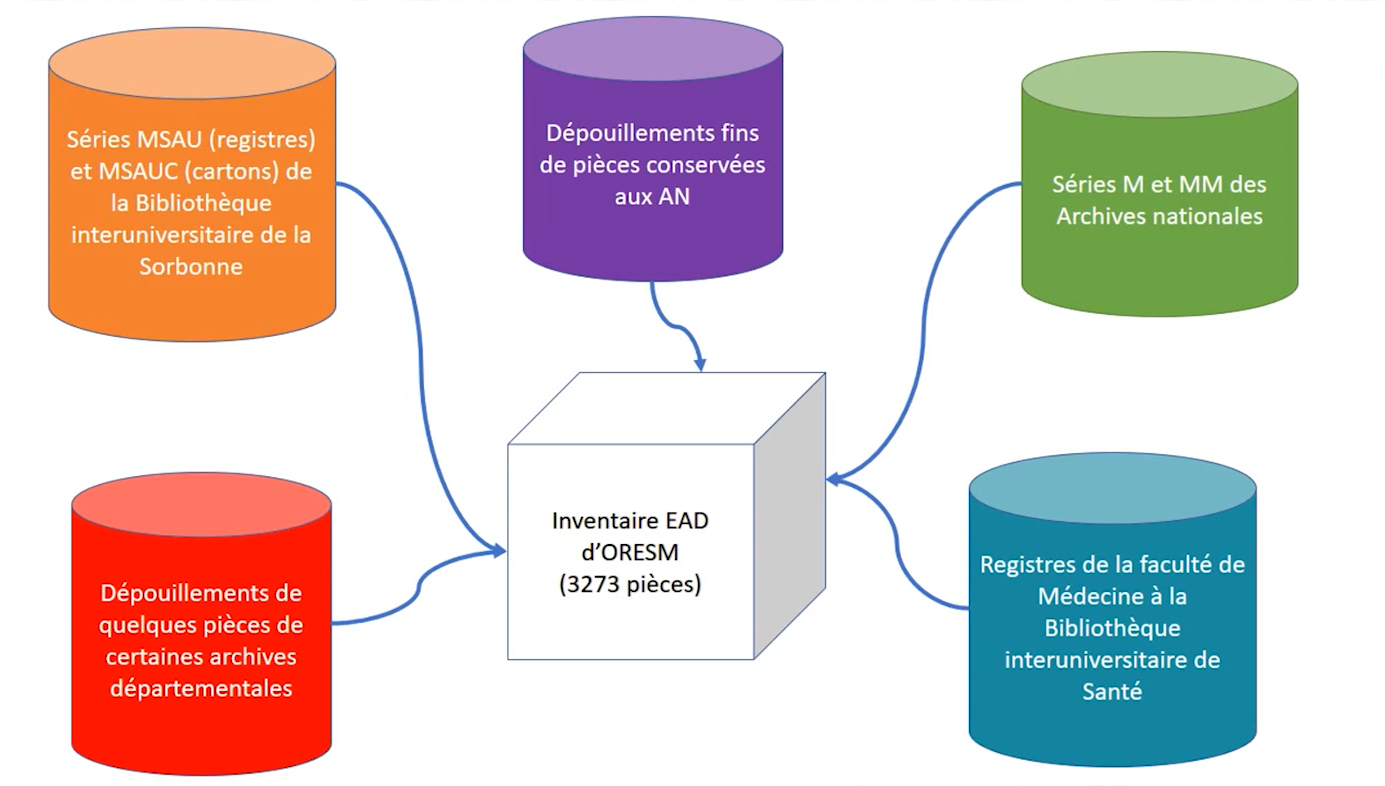
\includegraphics[width=0.8\linewidth]{images/Visualisation inventaire.png}
    \caption{Représentation du regroupement virtuel des notices archivistiques dans un même instrument de recherche.}
    \label{fig:visualisation-inventaire}
\end{figure}
\subsection{Dépouillements d'archives}
Lors de la construction de l'inventaire par Arsène un constat a été fait concernant les notices. Leurs contenus ne répondaient pas aux besoins des enjeux scientifiques du projet, notamment en ce qui concerne les entités nommées. Grâce à un financement du Labex Hastec la BIS a décidé de recruter Louise Gousseau, archiviste, afin de mener une campagne de dépouillements. Cette campagne a permis d'extraire des documents originaux les informations que le conseil scientifique a jugées nécessaires au projet. Le projet ORESM a pour ambition de faire dépouiller l'ensemble du fonds d'archives de l'ancienne université de Paris. Nous reviendrons en détail sur ces dépouillements, puisque les données produites sont au cœur des réalisations de ce stage.
\subsection{Preuve de concept de 2021}
Florence Clavaud a réalisé en 2021, sur une courte période de temps, une preuve de concept visant à démontrer la faisabilité et l'intérêt de la sémantisation des données ORESM dans un graphe de connaissance\footnote{Voir le support utilisé pour présenter cette preuve de concept lors d'une \href{https://oresm.hypotheses.org/files/2022/03/ORESM_JE_26112021_JFMoufflet_FClavaud-3.pdf}{journée d'étude en 2021.}}.  L'idée de cette preuve de concept était de produire ce qui va constituer le coeur du futur portail, à partir de l'ensemble des données disponibles dans les divers formats utilisés (EAD, Excel, référentiel Studium Parisiense). Pour cela il fallait choisir ou définir un modèle unique qui garantisse un haut niveau de granularité et d'exploitabilité, et qui permette par la suite de réutiliser les données. Les technologies sémantiques paraissaient une bonne méthode. Cette preuve de concept a posé les bases du traitement qui sera réalisé sur les données, et présenté dans ce mémoire. Le stage a étendu cette preuve de concept dans sa profondeur et sa portée. Nous reviendrons largement dans les parties suivantes sur celle-ci.
\part{Transformations des méta-données archivistiques en RDF}
\chapter{Origine des métadonnées}
La preuve de concept de 2021 avait été faite à partir des métadonnées produites pendant le travail de dépouillement de 188 documents, provenant du collège des Cholets. Depuis 2021 les dépouillements ont continué sur les archives de douze autres nouveaux collèges. Pour accélérer le processus, la méthodologie de dépouillement a été revue, ce qui  a permis de multiplier le nombre d'actes dépouillés par Louise Gousseau par cinq. Ce changement de méthodologie, très positif pour l'avancement du projet a permis de dépouiller 1441 pièces d'archives, issues de treize anciens collèges parisiens. Certains collèges, comme le collège d'Arras n'ont donné que quelques pièces quand d'autres, comme le collège de Fortet ou le collège du Cardinal-Lemoine, ont donné plus de 300 pièces. Cependant, cette méthodologie, plus simple, a produit des métadonnées moins riches que celles relatives aux 188 premières pièces et entraîne un écart qu'il faudra prendre en compte.
\par
Avant de présenter les métadonnées, il convient de rappeler ce qu'est un collège à l'époque médiévale et l'intérêt qu'ont les archives de ces institutions pour le projet ORESM. Le collège du Moyen Âge, bien loin du lieu d'enseignement qu'il est maintenant, est à l'origine un lieu d'hébergement pour étudiants pauvres. Ces établissements sont mis à disposition, de ceux qu'on appelle communément des boursiers, par des riches bienfaiteurs. La vie au sein du collège est réglée par des statuts que le fondateur impose aux étudiants pour donner un cadre propice à l'érudition. Le premier collège à apparaître à Paris est le collège des Dix-Huit fondé en 1180, peu de temps après l'émergence non officielle de l'Université de Paris. Tout au long du \textsc{XIII}\ieme{} et \textsc{XIV}\ieme{} siècle, le nombre de fondations de collège va croître, suivant et confirmant l'affirmation de la ville de Paris comme ville d'enseignement renommée. A la fin du \textsc{XIV}\ieme{} siècle la majorité des collèges parisiens sont déjà fondés, on en compte une cinquantaine et ce chiffre n'ira pas bien plus haut, le grand mouvement de fondation étant déjà passé. Bien souvent, les collèges accueillent des étudiants originaires d'une même région, comme le collège de Bayeux pour les étudiants normands. Avec la tenue de liste des étudiants boursiers, les archives de ces collèges sont de formidables sources d'enrichissement pour les recherches prosopographiques relatives à l'université de Paris. La majeure partie de ces archives (tout comme les archives de l'université proprement dite) est actuellement conservée aux Archives nationales dans la série M/MM pour les archives historiques majeures (les actes de fondations, les statuts, les dotations), la série H pour les archives comptables (quittances, redevances, livres de comptes)  et la série S sur les titres fonciers. Actuellement seule la série M/MM a été dépouillée ainsi que 180 documents conservés aux archives départementales de l'Oise et de la Seine-et-Marne, et 70 documents de la BIS.
\section{La méthodologie}
Cette méthodologie a été établie par le conseil scientifique du projet avec le groupe de travail Métadonnées pour répondre aux enjeux scientifiques. Une large part est consacrée à l'historique de conservation du document, ses anciennes cotes, ses lieux de conservation, les inventaires dans lesquels il apparaît. Ces informations serviront à comprendre la dynamique de production, de stratification et donc l'histoire du fonds de l'université de Paris aujourd'hui démembré. Il a été également décidé de relever les noms de personnes qui apparaissent dans le document, leurs rôles, les lieux de passage des actes, le nombre de noms présents. Toutes ces données pourront enrichir à terme la base \textit{Studium Parisiense} et accompagner les scientifiques dans leurs recherches prosopographiques.
\par
Il avait été décidé de découper le travail de l'archiviste en deux phases. Une première phase devait être réalisée à partir des documents originaux dans leur lieu de conservation (majoritairement les Archives nationales). Les informations uniquement disponibles sur les originaux devaient alors être relevées, par exemple le lieu de passage de l'acte en forme littérale s'il était trouvable, la date de l'acte en forme littérale, les mentions dorsales. Puis, lors d'une deuxième phase, l'archiviste devait compléter ses données directement dans les locaux de la BIS, en opérant un travail de normalisation comme la normalisation de la date, la normalisation des lieux, la récupération des lieux cités dans l'analyse, etc. Cette deuxième phase de travail n'a été que partiellement réalisée puisque la personne à qui ce travail avait été confié (Louise Gousseau) a quitté le projet en janvier 2023. Parallèlement aux dépouillements, Jean François Moufflet intégrait dans un fichier Excel des notions concernant les types, formes et états des documents dépouillés, en leur assignant des définitions et des références. L'objectif de ce travail est d'intégrer ces données au référentiel des types de documents des Archives nationales, afin par la suite de pouvoir lier ce référentiel à notre graphe de connaissance. Ce travail d'intégration de ces nombreux nouveaux concepts dans le référentiel des AN sera réalisé par Florence Clavaud au Lab des AN.
\par
Finalement la majorité des dépouillements se sont faits conformément à une méthodologie qui établissait 49 champs\footnote{L'ensemble de la méthodologie est en premier annexe de ce mémoire.\ref{methodologie}} à renseigner par acte. Si une partie de ces champs concerne directement les documents, d'autres décrivent le contexte de création des pièces dépouillées. Il font référence à d'autres entités (ou objets d'intérêt) que les documents eux-mêmes, ainsi qu'on pourrait le dire dans un graphe de connaissance. Ainsi, par exemple, y trouve-t-on mentionnés des personnes, les lieux et des institutions. Mais avant d'arriver au stade du graphe il a fallu saisir les données dans un format plus traditionnel.

\section{Le format tabulaire}
Pour saisir ces données, il a été décidé d'utiliser un tableau Excel pour chaque collège. Ce format a été choisi pour son côté pratique, il est facile à prendre en main et très répandu. Le format tableau permet d'exprimer de manière satisfaisante les informations récoltées lors des dépouillements. Les tableaux sont créés automatiquement à partir des inventaires déjà existants ; ils sont donc pré-remplis d'informations déjà relevées dans les inventaires, comme la cote, l'identifiant de la notice descriptive dans l'inventaire d'origine, une analyse et une date (pas toujours normalisée). De cette manière on peut estimer le temps que prendra le dépouillement des actes d'un collège étant donné qu'on peut avoir une idée approximative du nombre de pièces que l'archiviste aura à décrire. En suivant la méthodologie, l'archiviste donne une structure homogène à l'ensemble des tableaux, ce qui est essentiel pour exécuter le traitement ultérieur sur les données qu'il saisit. Une ligne du tableau représente un document décrit, les colonnes étant les informations relatives à ce document. Il faut donc bien comprendre que chaque ligne est indépendante l'une de l'autre et se suffit à elle-même dans ce format. C'est ultérieurement que se feront des regroupements ; ainsi, par exemple, quand l'archiviste indique la cote d'une pièce dans la colonne \textbf{Cote actuelle} et que sur une autre ligne il indique cette même cote dans la colonne \textbf{Acte original cote actuelle}, il en résulte que la même cote est mentionnée plusieurs fois. C'est par un traitement ultérieur qu'il sera procédé à un regroupement des données relatives à cette unique entité cote, qui sera reliée aux actes qu'elle concerne par diverses relations.
\par
L'objectif de ce travail est d'aller décrire les pièces d'une manière plus fine qu'elles ne le sont actuellement. La plupart des instruments de recherche produits par les archivistes aujourd'hui s'arrêtent au niveau du dossier, faute de moyens pour descendre au niveau de la pièce. La description analytique est réservée aux fonds les plus anciens (car les documents écrits sont plus rares pour ces époques que pour l'époque contemporaine), les plus remarquables ou aux contenus les plus diversifiés, comme celui de l'Université de Paris au Moyen Âge qui est l'objet de ce projet. Un projet de recherche comme ORESM peut donc constituer une occasion de procéder à une telle opération. Les inventaires des séries M et MM\footnote{\href{https://www.siv.archives-nationales.culture.gouv.fr/siv/IR/FRAN_IR_001382}{Permalien de l'inventaire de la série M/MM.}} des Archives nationales tels qu'ils sont disponibles actuellement pour les usagers décrivent quasi exclusivement des pièces. L'un des objectifs des dépouillements est d'enrichir ces inventaires pour pouvoir y disposer à terme d'une analyse beaucoup plus précise et détaillée que celles qui s'y trouvent déjà. Dans cette forme de saisie la pièce d'archive reste au centre des considérations, les liens qui peuvent apparaître entre les différentes pièces ou entre les éléments décrits s'ils existent ne sont pas explicites. 
\par
Le format tabulaire a cependant certaines limites qu'il a fallu contourner par la mise en place de règles. Voici plusieurs exemples pour illustrer ces limites. Tout d'abord, un tableau n'est pas adapté au cas où plusieurs valeurs doivent être saisies pour une donnée d'une nature spécifique. Or dans le cas des dépouillements opérés, il arrive souvent qu'on ait besoin de saisir plusieurs données de même nature (on peut citer le cas d'un document qui a plusieurs cotes anciennes). La solution trouvée dans ce cas a été d'utiliser le caractère \textbf{"|"} appelé barre verticale\footnote{Pipe en anglais.}. Quand il est utilisé, il sépare deux données de même nature mais indépendantes l'une de l'autre. C'est le seul caractère réservé lors de la saisie des données indépendamment de la colonne. 
\par
Mentionnons un autre facteur de complexité en prenant l'exemple des actes originaux : dans un cas normal l'archiviste indique dans les 4 colonnes prévues à cet effet l'analyse de l'acte original dont est tiré le document dépouillé (qu'il s'agisse d'un acte copié ou d'un vidimus), son lieu de passage, la date normalisée de cet acte et la cote actuelle de l'acte. Quand il n'y a qu'un unique acte original, cela fonctionne très bien. Mais il peut arriver qu'un document consiste en la copie de plusieurs actes originaux. Comment faire correspondre entre chaque colonne les bonnes informations entre elles ? Le choix a été fait de se baser sur la position de l'information dans la case, la première valeur de la ligne dans la colonne analyse de l'acte original correspondra avec la première valeur de la date de l'acte original etc, le tout séparé par des barres verticales.
\par
\begin{figure}[!h]
    \centering
    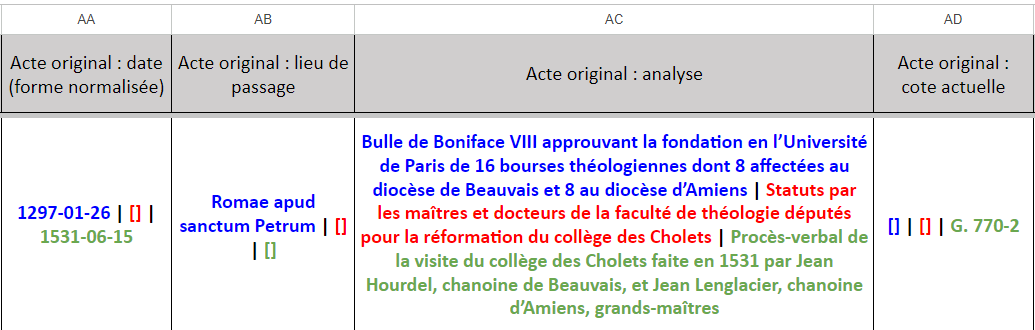
\includegraphics[width=1\linewidth]{images/tableau-positions-originaux.png}
    \caption{Capture d'écran d'une ligne d'un tableau pour illustrer l'importance de la position. Chaque couleur représente un acte.}
    \label{fig:position-tableau-couleur}
\end{figure}
Il en résulte qu'il faut également trouver le moyen de représenter l'absence de valeur. Puisque la position est importante on doit pouvoir la conserver, même quand il y a une valeur nulle ; c'est là qu'intervient une autre chaîne de caractères récurrente formée d'un crochet gauche et d'un crochet droit \textbf{"[]"}  qu'on appellera "crochets vides". Cette chaîne de caractères est utilisée tout au long des dépouillements pour représenter l'absence de valeur, quand une donnée était attendue, afin de respecter le schéma de saisie. 
\par
Un dernier exemple, cette fois-ci concernant les personnes. La méthodologie demande d'extraire les noms des personnes, leurs occupations/activités et leurs rôles par rapport au document analysé (auteur, rédacteur, témoin etc) le tout dans une seule colonne. On a donc l'expression de plusieurs valeurs (puisque qu'il est courant que plusieurs personnes soient impliquées dans un acte) et des valeurs de différentes natures. Pour permettre de retrouver quelle information est de quel type, il a été décidé de les ordonner selon un schéma que doit respecter l'archiviste : celui-ci indique en premier et entre crochets le rôle de la personne, puis son nom et entre parenthèses ses occupations/activités. Comme ces dernières peuvent être multiples et qu'on ne peut pas utiliser une barre verticale, on les sépare par un \# (dièse).
\par
Toutes ces consignes de saisie, indispensables à un tel niveau de granularité, visent à permettre aux traitements automatiques ultérieurs sur les données de produire des résultats de qualité. Mais cela exige une attention accrue de la part de la ou des personnes chargées du dépouillement et de la saisie des données. D'ailleurs requérir un tel niveau d'attention a pu entraîner certaines erreurs, qu'il nous a fallu corriger. Ces erreurs sont inévitables lorsqu'une personne humaine est en charge de la saisie. 
\chapter{Sémantiser pour exploiter les données}
Pour pouvoir exploiter les données issues des dépouillements fins, il a été décidé de se baser sur un modèle d'encodage récent qui utilise les technologies du web sémantique. 
\subsubsection*{Les technologies du web sémantique}
Les technologies du web sémantique existent depuis 1997\footnote{\href{https://www.w3.org/2001/sw/wiki/Main\_Page}{https://www.w3.org/2001/sw/wiki/Main\_Page}}, instaurées et maintenues par le W3C elles sont constituées :
\begin{itemize}
    \item Du langage RDF, qui définit une syntaxe pour décrire des entités par des phrases en trois parties sujet/verbe/objet.
    \item Des langages RDFS/OWL qui permettent de produire des modèles de données ou ontologies définissant des catégories d'objets (classes), leurs caractéristiques intrinsèques et les relations qui sont susceptibles de les lier entre elles.
    \item Un langage de requête pour interroger ces données, SPARQL, que nous présenterons plus tard.
\end{itemize}
Ces technologies s'appuient sur l'architecture du Web ; une entité est identifiée par son URI. Pour être plus précis les phrases, appelées triplets, sont composées d'un sujet, d'un prédicat et d'un objet. Un ensemble de triplets est appelé un graphe orienté. 
\par
Les avantages de ces technologies sont, en premier les possibilités que permet la définition des ontologies\footnote{Une ontologie est la définition informatique d'un ensemble de règles et de relations sémantiques pour représenter un modèle de données propre à un domaine identifié.}. Pour peu qu'on les maîtrise, ces technologies permettent de modéliser n'importe quel domaine de connaissances si on est capable de bien identifier les catégories d'entités (classes) qui le composent et les relations nécessaires. Cela permet de gérer la granularité de son modèle de données. Le second avantage porte sur la structure des données ; elles ne sont plus figées dans une arborescence bidimensionnelle, comme elles peuvent l'être dans l'inventaire en EAD. On passe à un graphe multi-dimensionnel. Troisièmement, l'interopérabilité des données est un fondement du web sémantique. En utilisant des URIs pour identifier les entités on peut référencer ces entités et donc établir des relations entre ces entités, y compris des relations d'équivalence. Si par ailleurs on partage les mêmes modèle de référence (ontologies), ou qu'on articule entre eux plusieurs modèles, on pourra plus facilement lier des jeux de données entre eux, échanger des données.

\section{Utilisation de RiC-O}
\subsection{L'arrivée du web sémantique dans les archives}
 Le développement de la science ouverte et de l'open data dans le monde des humanités numériques, lors de la décennie passée, a entraîné un regain d'intérêt pour ces technologies qui ont commencé à être utilisées par différents milieux comme les bibliothèques et les musées. Depuis 2013 un groupe de travail de l'ICA (International Council on Archives) dont fait partie Florence Clavaud, l'EGAD (Expert Group on Archival Description) développe le modèle conceptuel RiC-CM pour représenter les "Records in Contexts", plus clairement pour décrire les documents d'archives dans leurs contextes de création, d'accumulation et d'utilisation au fil du temps. Ce modèle conceptuel fait apparaître quatre entités essentielles : le Record Resource, l'Instantiation\footnote{L'entité Instantiation de RiC représente la manifestation physique d'un Record Resource. Un Record Resource a forcément eu une Instantiation associée lors de sa création mais celle-ci peut avoir été perdue. Les relations associées à l'Instantiation concernent son lieu de conservation, les propriétés physiques du document, son support, les autres manifestations dérivées de l'Instantiation (par exemple une numérisation).}, l'Agent et l'Activity. L'entité Agent est une super entité qui englobe les entités Corporate Bodies, Persons, et Families\footnote{Ces entités existent également dans la norme de description ISAAR(CPF), norme utilisée pour décrire les notices d'autorités archivistiques, relatives aux collectivités, aux personnes et aux familles.}. L'un des enjeux du développement de RiC était de remplacer les quatre standards actuels utilisés dans la description d'archives (et notamment le standard ISAD G, qui a pour norme d'encodage la DTD EAD) par un seul. On peut également souligner l'existence de l'entité Place qui représente un lieu. Vu la part importante d'informations relevées sur les lieux lors des dépouillements (les noms des lieux de passage ou des lieux cités dans l'analyse des actes sous différentes formes, leurs coordonnées, les pays) cette entité sera essentielle pour représenter nos données. Dans une moindre mesure c'est la même chose pour les dates, qui sont représentées par des entités Date dans RiC-CM. Les éléments de datation sont exprimés de trois manières différentes dans les fichiers de dépouillement, sous forme littérale, rédigée et normalisée. Il était donc nécessaire d'avoir ces entités dans le modèle conceptuel afin d'exprimer ces données. La première version de RiC-CM est publiée en août 2016. En février 2021 l'ontologie RiC-O 0.2 est également publiée. Cette ontologie est une transposition technique, en OWL, du modèle conceptuel RiC-CM. C'est l'ontologie de référence pour produire des métadonnées archivistiques en RDF conformes à RiC. La création de cette ontologie nourrit la réflexion sur la logique de RiC-CM. La version 1.0 de RiC-CM et RiC-O doit être publiée à la fin de l'année 2023.

\par
\begin{figure}[ht]
    \centering
    \includegraphics[width=0.8\linewidth]{images/Hiérarchie des classes RiC.png}
    \caption{Tableau hiérarchique des classes du modèle RiC-CM}
    \label{fig:tableauclassericcm}
\end{figure}
\subsection{Un modèle déjà utilisé qui fait ses preuves}
Il s'agit donc d'un modèle encore très récent. Cependant les Archives nationales ont été pionnières dans l'utilisation de RiC, dès 2015. Le Lab a commencé par des expérimentations, puis a lancé plusieurs projets à plus grande échelle, soit directement pour le compte des Archives nationales soit en mettant à disposition son expertise dans des projets extérieurs\footnote{Florence Clavaud.\href{https://rec.unil.ch/videos/florence-clavaud-ric-aux-archives-nationales-de-france-enjeux-realisation-perspectives/}{Records in Contexts (RiC) aux Archives nationales de France : enjeux, réalisations, perspectives. Demi-journée d'information} \textit{RIC (Records in Contexts). Quels changements et quelles perspectives ?}, Association vaudoise des archivistes (AVA), Dec 2022, Lausanne (CH), Suisse. ⟨hal-03957469⟩}. Parmi les projets en cours, soulignons que le Lab a sémantisé tous les référentiels des Archives nationales, avec l'ontologie RiC-O\footnote{\href{https://github.com/ArchivesNationalesFR/Referentiels}{https://github.com/ArchivesNationalesFR/Referentiels}}, en particulier celui des types de document dont nous avons parlé, celui des supports et celui des langues. Ces référentiels ont été facilement intégrés au projet ORESM puisqu'ils suivent le même format que nos données. 
Les membres du groupe EGAD espèrent entraîner une transition vers Records in Context dans tout les services d'archives. Pour aboutir à ce résultat, les Archives nationales réalisent un logiciel nommé RiC-O Converter\footnote{\href{https://github.com/ArchivesNationalesFR/rico-converter}{https://github.com/ArchivesNationalesFR/rico-converter}} qui automatise la transformation des données encodées en EAD et EAC-CPF en données conformes à RiC-O. Ce logiciel a été utilisé pour transformer une partie des descriptions des archives notariales des Archives nationales lors de la réalisation en 2022 d'une plate-forme\footnote{\href{https://sparna-git.github.io/sparnatural-demonstrateur-an/index.html}{https://sparna-git.github.io/sparnatural-demonstrateur-an/index.html}} destinée à tester un éditeur visuel de requêtes SPARQL, Sparnatural, sur lequel nous reviendrons ultérieurement.




\section{Pourquoi étendre l'ontologie ?}
\subsection{Un modèle généraliste, des données spécialisées}
L'ontologie RiC-O comme nous l'avons vue est un modèle qui nous satisfait dans les classes et propriétés qu'il met à notre disposition. Pourtant, pour répondre à la granularité forte de notre gisement de données et pour prendre en compte les spécificités de l'analyse de pièces d'archives médiévales et l'histoire complexe de leur conservation, dans le cadre de ce projet, les relations proposées ne sont pas suffisantes. C'est ce qu'avait déjà estimé Florence Clavaud ; lors de la réalisation de la preuve de concept de 2021, elle avait commencé à lister et modéliser les relations supplémentaires nécessaires pour sémantiser les données de dépouillements. RiC-O par exemple n'a qu'une seule relation pour représenter le lien entre une Instantiation et un Agent qui a conservé ou qui conserve celle-ci, c'est la relation \textbf{has or had holder}\footnote{\href{https://www.ica.org/standards/RiC/ontology\#hasOrHadHolder}{https://www.ica.org/standards/RiC/ontology\#hasOrHadHolder}}. Avec les enjeux fondamentaux du projet, de suivre le parcours des archives et de savoir où et quand elles ont été conservées, il est nécessaire de dépasser cette simple relation qui ne précise pas si la conservation est passée ou actuelle. Même chose pour la relation entre une Instantiation et son Identifier\footnote{La classe Identifier dans RiC-O peut servir à représenter l'ensemble des combinaisons de symboles pour identifier une entité précise, dans notre modèle de données elle fait référence à la cote d'un acte. } \textbf{has or had identifier}\footnote{\href{https://www.ica.org/standards/RiC/ontology\#hasOrHadIdentifier}{https://www.ica.org/standards/RiC/ontology\#hasOrHadIdentifier}}; cette relation peut être utilisée pour relier une archive à sa cote, qu'elle soit actuelle ou passée. Or dans le cadre de notre projet nous avons besoin de distinguer ces deux cas. D'autant plus que la période d'utilisation de la cote est parfois spécifiée dans nos tableaux de dépouillements. Utiliser uniquement ces relations nous aurait fait perdre en précision, ce qui n'était pas envisageable.
\par
Par ailleurs, en ce qui concerne l'analyse diplomatique des documents, pour exprimer la tradition de ces actes nous avons besoin de relations plus précises que celles disponibles dans RiC-O. Pour le chercheur en histoire médiévale, et tout spécialement dans le cadre du projet ORESM, il est important de consigner les liens génétiques reliant les différents états d'un texte ; ceux-ci avaient donc été notés dans les tableaux de dépouillement et il était nécessaire de représenter ces liens avec le même niveau de précision que le spécifiaient ces tableaux. Pour les représenter, on ne peut pas simplement se contenter des relations mises à disposition par RiC-O. Par exemple, la relation \textbf{is copy of}\footnote{\href{https://www.ica.org/standards/RiC/ontology\#isCopyOf}{https://www.ica.org/standards/RiC/ontology\#isCopyOf}}
 permet de relier une copie à son original. Mais comment représenter la relation entre un vidimus et son original ? Même chose pour la relation entre un acte inséré ou un acte extrait, et l'original dont il est issu. Qu'en est-il de la relation de l'Agent aux pièces décrites ? Des notions comme le testateur ou le témoin d'un acte qui sont très importantes dans la période étudiée ne sont pas présentes dans RiC-O 0.2. Ce qui est normal, c'est un modèle qui est conçu avant tout pour être générique. Il offre des solutions pour la description d'archives, afin de répondre aux besoins de la majorité des cas, et surtout donne un cadre pour un étendre le modèle si nécessaire, et en cela il est déjà très utile. Il est évident que le niveau de description des dépouillements effectués dans le cadre du projet ORESM va bien au delà du niveau habituel, davantage encore si on ajoute la spécificité du vocabulaire médiéval. C'est pourquoi cette ontologie a été étendue, pour prendre en compte les relations identifiées comme manquantes et exprimer pleinement le niveau de granularité de notre gisement de données.
 \begin{figure}[!h]
     \centering
     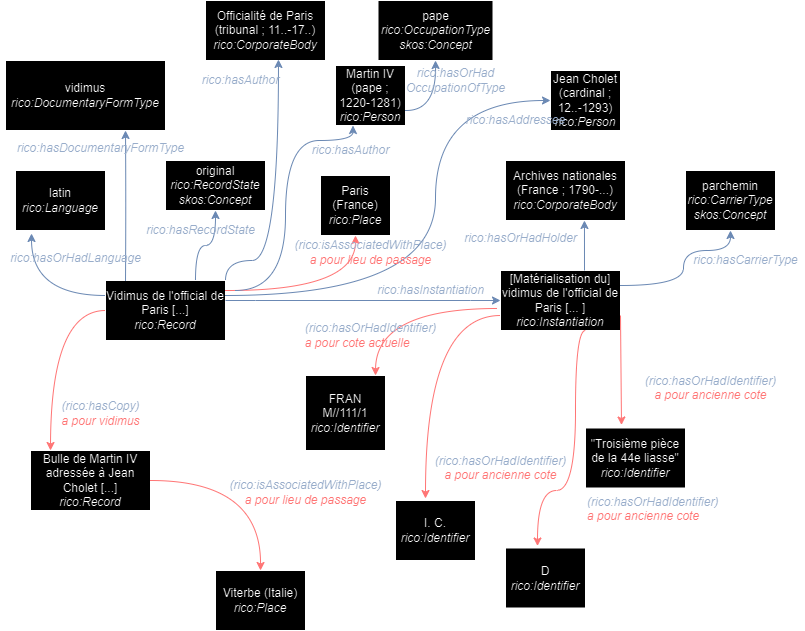
\includegraphics[width=0.8\linewidth]{images/visualisation relations manquantes.png}
     \caption{Visualisation réalisée par Florence Clavaud, pour sa preuve de concept de 2021 qui indique en rouge les relations nécessaires pour le projet ORESM qui n'existent pas dans RiC-O 0.2.}
     \label{fig:enter-label}
 \end{figure}
\subsubsection*{Protégé}
Le logiciel gratuit et open source d'édition d'ontologies Protégé est utilisé dans le cadre de ce projet. Il est développé par l'Université de Stanford. Il permet, avec une interface claire, de visualiser et d'éditer une ontologie. Il est très utilisé par les ingénieurs spécialistes du web sémantique grâce à sa facilité d'accès et l'interface de travail ergonomique qu'il propose. Dans les cas d'ontologies riches et complexes comme RiC-O, il est très utile de pouvoir les ouvrir et les modifier, à l'aide de cet outil, sans devoir impérativement éditer ces ontologies dans leur format source, en l'occurrence XML/RDF. Également en visualisant l'ontologie RiC-O dans Protégé on peut plus facilement appréhender les notions d'héritage. Grâce à cette vue on peut naviguer facilement et comprendre encore mieux les possibilités de RiC-O.
\begin{figure}[ht]
    \centering
    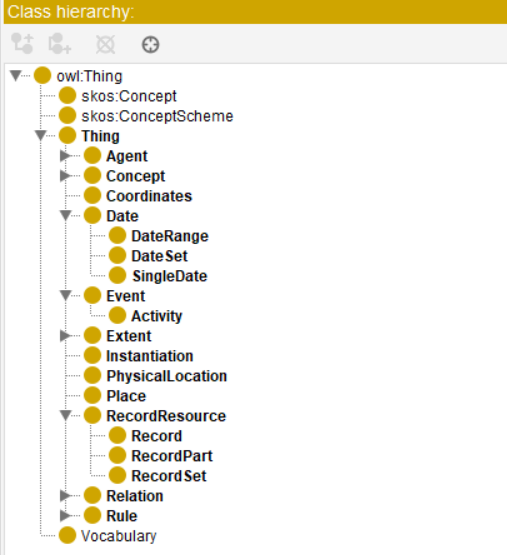
\includegraphics[width=0.6\linewidth]{images/Protégée Classes RiC-O.png}
    \caption{Capture d'écran de la visualisation hiérarchique des classes de l'ontologie RiC-O dans Protégée}
    \label{fig:protegee_classe_rico}
\end{figure}
\subsection{Extension de RiC-O, l'ontologie ORESM}
C'est donc en utilisant Protégé qu'a été élaborée l'ontologie ORESM. Celle-ci reprend l'ensemble des classes et des relations de RiC-O, et lui ajoute de nouvelles relations et une seule classe, dite de relation que nous allons présenter plus loin. Au total 42 nouvelles relations\footnote{Ce nombre prend en compte les relations et leurs inverses.} ont été ajoutées, ainsi que 17 datatype properties\footnote{Une datatype property en OWL est une relation qui lie une entité à une valeur textuelle sans URI. On peut dire que ce sont les attributs de l'entité.} Il a été décidé de libeller et de décrire ces relations en français notamment pour différencier les relations de celles de RiC-O qui sont en anglais, mais également par souci purement pratique : cette ontologie étant centrée sur la description d'archives françaises avec des acteurs français, il n'y avait pas d'intérêt à insérer de l'anglais dans nos travaux. 
\par
Nous évoquions plus haut les relations manquantes pour exprimer le lien entre une institution de conservation et l'Instantiation d'un document, en distinguant une relation passée ou présente. La solution a été de créer deux relations qui sont des sous-propriétés de la relation \textbf{has or had holder}\footnote{\href{https://www.ica.org/standards/RiC/ontology\#hasOrHadHolder}{https://www.ica.org/standards/RiC/ontology\#hasOrHadHolder}}, l'une au passé la relation \textbf{a conservé} et son inverse \textbf{a été conservé par}, et l'autre au présent \textbf{conserve actuellement} et son inverse \textbf{est conservé actuellement par} . Les deux relations inverses sont sous-propriétés de \textbf{'is or was holder of'}\footnote{\href{https://www.ica.org/standards/RiC/ontology\#isOrWasHolderOf}{https://www.ica.org/standards/RiC/ontology\#isOrWasHolderOf}} elle même relation inverse de \textbf{has or had holder}.
\par
Pour ce qui est de la relation entre la cote et une pièce d'archives à laquelle elle se rapporte, deux solutions ont été trouvées. La première comparable au cas des institutions de conservation, a consisté à créer quatre relations d'entité à entité, qui sont des sous-propriétés de \textbf{has or had identifier}\footnote{\href{https://www.ica.org/standards/RiC/ontology\#hasOrHadIdentifier}{https://www.ica.org/standards/RiC/ontology\#hasOrHadIdentifier}} et son inverse. Mais parfois, comme nous l'avons dit, la cote dans le tableau de dépouillement est associée à un élément de datation précis. Or il n'est pas possible, dans une ontologie OWL de qualifier un verbe (une relation). 
\par
Ce que nous voulions avec notre modèle de données, était d'exprimer la relation entre par exemple la cote \textit{BB : I : 13e} et le document coté, en exprimant que cette cote a été utilisée au \textsc{XVIII}\ieme{} siècle. C'est là que les classes de relation fournies par RiC-O sont très intéressantes ; ce sont des classes qui représentent des relations en tant qu'entités. Elles ont les caractéristiques informatiques d'une entité, c'est à dire qu'on peut utiliser des propriétés pour les décrire ; mais elles servent de noeud intermédiaire entre les entités qu'elles relient. C'est pour l'instant la seule classe de relation qui a été ajoutée à l'ontologie. Bien que très utiles, de telles classes doivent être évitées si possible, car bien que l'on gagne en précision, on augmente de manière conséquente le nombre de triplets. Nous envisageons toutefois de créer une classe de relation pour relier le lieu de passage d'un acte et celui-ci, afin d'exprimer la forme littérale d'un lieu par rapport à l'acte dans lequel il apparaît. Ce sera une préoccupation future, une fois que le travail de normalisation des noms de lieu sera fait.
\begin{figure}[h]
    \centering
    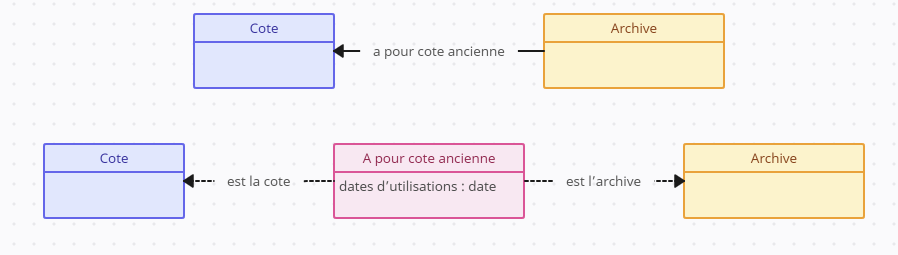
\includegraphics[width=0.9 \linewidth]{images/Classe de relation.png}
    \caption{Représentation UML d'une classe de relation par rapport à une relation simple pour le cas des cotes anciennes.}
    \label{fig:classe_relation}
\end{figure}
\par
Pour résumer nous avons créé une ontologie ORESM en l'articulant avec le cadre générique que constitue RiC-O. Tous les composants que nous avons créés dans cette ontologie sont définis comme des sous-composants RiC-O. Notre modèle est donc en conformité avec l'ontologie qu'il étend, ce qui garantit pour l'avenir l'interopérabilité de nos données avec d'autres jeux de données utilisant RiC-O. Si l'on veut faire rentrer nos données dans un ensemble utilisant RiC-O c'est facilement faisable.  Comme chacune des nouvelles propriétés définies dans l'ontologie ORESM est déclarée comme étant une sous-propriété de RiC-O, un raisonneur connaissant OWL pourra, chaque fois qu'une telle propriété sera instanciée dans nos données, en déduire le triplet utilisant la super-propriété RiC-O. Il sera même ainsi possible, par exemple, au portail FranceArchives\footnote{Le portail FranceArchives a effectué une transition de ses données vers RiC-O en septembre 2023.} d'utiliser les données ORESM si à l'avenir il souhaite les récupérer pour les agréger à celles conformes à RiC-O qu'il utilise déjà ; il lui suffira de n'exploiter que ces triplets conformes à RiC-O, en perdant ainsi, bien sûr, en précision.  Un renvoi vers le futur portail ORESM permettra à l'usager de revenir aux données source.

\section{Construction d'un modèle}
Pour préparer la transformation des données il a été nécessaire d'interroger le contenu des colonnes de nos tableaux de dépouillements. Comme nous l'avons détaillé en quelques exemples précédemment, il fallait faire correspondre une relation ou une entité de notre ontologie avec les données qui ont été dépouillées par l'archiviste, c'est ce qu'on appelle un \textit{data mapping}. Le but principal étant de voir si tout pouvait être exprimé en RDF nous avons, pour chaque colonne, étudié les différentes formes que pouvaient prendre les valeurs et comment les exprimer dans notre ontologie. C'est lors de cette étape que l'ontologie ORESM a été conçue en parallèle, afin de trouver une solution quand RiC-O n'était pas suffisant. Nous avons donc, suivant les conseils de Florence Clavaud, élaboré un \textit{tableau de mapping}\footnote{Ce tableau de mapping est inspiré de la documentation de RiC-O Converter, qui spécifie comment des métadonnées encodées en EAD sont transformées en données RiC-O, disponible sur le github \href{https://github.com/ArchivesNationalesFR/rico-converter/blob/master/docs/EAC_to_Ric-O_0.2_documentation.xlsx}{https://github.com/ArchivesNationalesFR/rico-converter/}. \textit{(Visité le 12/10/2023)}} qui synthétise cette réflexion. C'est un tableau à six colonnes ; chaque ligne représente une colonne des tableaux de dépouillements. On y donne un exemple de valeur que peut prendre une cellule dans ce tableau d'origine, puis on représente comment cette valeur sera exprimée en RDF, on y consigne une remarque si besoin ; une dernière colonne précise, de façon rapide et simple, quelle classe ou datatype property RiC-O est employée. Ce tableau de mapping est en annexe de ce mémoire. \ref{mapping}
\chapter{Transformation des données}
Toujours en partant de la preuve de concept réalisée par Florence Clavaud, la transformation automatique des données se fait en utilisant un unique programme écrit dans le langage XSLT 2.0.\footnote{Lien vers \href{https://www.w3.org/TR/xslt20/}{la spécification W3C.}} Le choix de ce langage tient au format de sortie choisi qui est RDF/XML. XSLT est une technologie extrêmement performante quand il s'agit de transformer du XML ou du texte en XML.
\section{Transformation à partir des tableaux Excel}
\subsection{Logique de transformation}
Pourquoi partir des données des fichiers Excel, et ne pas utiliser le logiciel RiC-O Converter sur les données en EAD ? En effet l'inventaire virtuel encodé en EAD contient déjà les données saisies dans les fichiers Excel de dépouillements. Tout d'abord, utiliser le logiciel RiC-O Converter aurait été complexe puisqu'il ne connaît pas l'extension de RiC-O que nous avons produite, il aurait donc fallu que nous nous l'approprions et l'adaptions à nos besoins. Et pourquoi ne pas partir du fichier EAD et faire notre script qui utilisera l'ontologie ORESM ? En fait, il s'avérait nettement préférable de partir de la source Excel : le fichier EAD résultait déjà d'une transformation simplifiant de beaucoup la structure initiale des données. Finalement il était plus naturel et plus rapide de partir de la base déjà fournie par la preuve de concept proposée par Florence Clavaud. 
\par
Pour gagner du temps nous avons utilisé le logiciel Oxygen\footnote{C'est à partir de la version 23 qu'Oxygen propose cette fonctionnalité directement incluse, pour des versions plus anciennes il faudra installer un add-on.} qui permet de transformer un fichier Excel en format XML. On se retrouve avec un fichier ayant un élément racine qui contient pour chaque ligne du tableau original un élément XML \textbf{<document>}. Dans chacun des éléments \textbf{<document>}, on trouve pour chaque colonne du tableau Excel, un élément du même nom qui contient la valeur de la cellule correspondante dans le tableau.
\begin{figure}[!h]
    \centering
    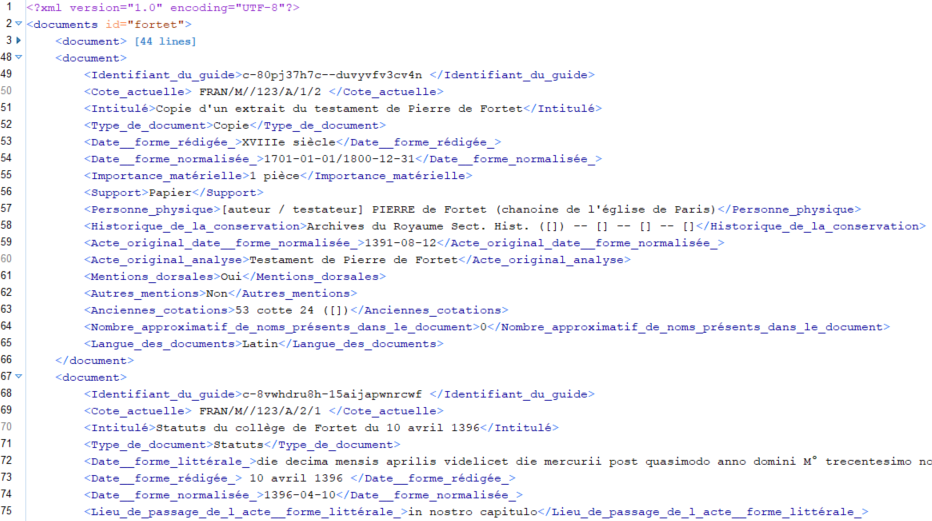
\includegraphics[width=1\linewidth]{images/tableau-fortet-xml.png}
    \caption{Premières lignes du fichier XML issu du tableau de dépouillement du collège de Fortet.}
    \label{fig:xml-fortet}
\end{figure}

\subsection{Organisation à la sortie du script}
Tout l'objectif du script est d'extraire de ces fichiers tabulaires la description des entités qui s'y trouvent mentionnées et qui sont dignes d'intérêt pour le projet, et les relations qui lient les entités entre elles pour former un graphe orienté. On change complètement la manière d'organiser les données. Selon l'approche déjà suivie par Florence Clavaud pour sa preuve de concept, le script traite en premier lieu les entités de contexte et seulement à la fin du processus, les documents. La relation entre ces entités de contexte et le document décrit est exprimée au moment où les entités de contexte sont traitées. Pour bien différencier les types d'entités chacun bénéficie de son propre fichier de sortie. Il en résulte :
\begin{itemize}
    \item Un fichier pour les personnes physiques (3478 entités rico:Person créées).
    \item Un fichier pour les personnes morales (102 entités rico:CorporateBody).
    \item Un fichier pour les lieux (314 entités rico:Place).
    \item Un pour les cotes anciennes et un pour les cotes actuelles (2745 rico:Identifier).
    \item Un fichier pour les types d'activité, de titre, ou de fonction (929 rico:OccupationType).
    \item Un fichier pour les dates (1715 entités date).
    \item Un fichier unique pour les statuts et types de documents (120 entités rico:Type).
\end{itemize}
\par
L'URI de chaque entité créée par le projet ORESM commence par une chaîne de caractères invariante déclarée dans les fichiers XML/RDF de sortie, \og  http://data.oresm.fr\fg. Dans le cas des entités ci-dessus l'URI est suivi par la classe puis le nom de l'entité. Donc  l'URI du lieu Paris est \og http://data.oresm.fr/place/Paris\fg. 
\par
Pour l'entité représentant le document d'archives le fichier de sortie est individualisé. Pour nous retrouver dans la masse de ces fichiers (1445 fichiers, un fichier par document dépouillé) il a fallu trouver un moyen pour les différencier. Nous avons décidé de créer une clé d'identification à partir du numéro d'ordre de la ligne décrivant le document dans le tableau, et du nom du fichier d'origine. Ainsi le document  qui est décrit à la ligne 145 du fichier relatif au collège de Fortet est décrit en RDF dans le fichier de sortie \og document-fortet-145\fg . C'est un très bon moyen court et efficace pour se retrouver en utilisant autre chose que la cote ou l'analyse. C'est d'ailleurs sur cette même logique que sont construits les URI des documents. Toujours en reprenant l'exemple précédent, l'URI des deux entités RiC-O représentant le document décrit à la ligne 145 est recordResource/or-fortet-145 et instantiation/or-fortet-145 (le radical or signifie ORESM). Ce système d'identification permet de cibler un document très précisément, et de le retrouver très rapidement, notamment dans le script, lorsqu'on exprime la relation entre l'entité de contexte et le document, il suffit simplement d'identifier la ligne.


\section{Commentaires}
\subsection{Réussites}
En premier lieu il est important de souligner la réussite de cette étape. Le script XSLT remplit parfaitement son mandat. En suivant le tableau de mapping, chaque cellule d'origine des tableaux est transformée en RDF suivant l'ontologie RiC-O/ORESM. Le script produit les fichiers de sortie en moins de 10 secondes. C'est la une force de XSLT, la vitesse d'exécution. La plus grosse difficulté a été de gérer les actes et leurs originaux, notamment pour éviter les doublons, quand deux actes sont la copie d'un même original. En quelques mots, quand un acte est issu d'un original également décrit via une ligne d'un fichier Excel, on peut regrouper les données décrivant cet unique original et ne créer au final qu'une seule description de cet original, en utilisant les champs concernant sa cote. Quand l'original n'est pas dans les actes dépouillés alors il est créé une entité RecordResource représentant l'acte original mais sans entité Instantiation associée. C'est ce que nous avons appelé un acte \og virtuel\fg. 
\par
Mais il est possible que plusieurs actes soient tirés d'un même original, pas encore dépouillé, voire même perdu. Pour éviter les doublons d'actes virtuels, il a été décidé de comparer les données \textbf{Acte\_original\_analyse} et \textbf{Acte\_original\_date}. Si l'archiviste a relevé la même date et la même analyse pour la pièce originale de deux (ou plus) documents lors du dépouillement, alors on considère qu'ils sont issus de la même pièce. Pour illustrer cette situation prenons les pièces ayant pour cote, l'une \textbf{FRAN/M//74/9} et l'autre \textbf{FRAN/M//74/10}. Pour ces deux pièces l'archiviste a relevé que l'original était daté de \textit{1263-05-04} et a rédigé une analyse identique \footnote{\textit{Privilège donné aux pauvres maîtres de Sorbonne par le pape Urbain le 4 des nones de mai l’an II de son pontificat de construire une chapelle et d’y célébrer les offices.}}. Dans un tel cas, le script ne crée qu'un unique acte virtuel. Cette logique permet de de faire émerger des clusters de relations. Pour donner une idée, dans nos données, un acte virtuel a pu être lié à neuf actes dépouillés. Il a aussi été décider d'effectuer la normalisation\footnote{Au format ISO 8601 : yyyy-mm-dd} des formes rédigées des dates quand celles-ci répondent à un certain schéma, identifié à l'aide d'expressions régulières\footnote{Les expressions régulières sont des motifs de recherche qui permettent de décrire des modèles de chaînes de caractères. Voir la page wikipédia dédiée \href{https://fr.wikipedia.org/wiki/Expression\_r\%C3\%A9guli\%C3\%A8re}{https://fr.wikipedia.org/wiki/Expression\_régulière}.}. Le script ne réalise donc pas uniquement une transformation mais effectue un traitement et une interprétation des données quand il est intéressant de le faire.

\subsection{Limites}
Évidemment on ne peut pas tout faire dans un unique script. Certains traitements qui auraient pu être envisagés ont été laissés de côté. 

\subsubsection{Pas de réconciliation précise des entités nommées}
Concernant les entités nommées, la seule réconciliation opérée consiste à regrouper les entités sur la base d'une égalité parfaite des valeurs qui les concernent. Les entités de type personne (appartenant à la classe Person de RiC-O) sont regroupées sur leurs noms mais aussi leurs occupations. Ainsi un \og Germain Gouffe \fg identifié dans un acte comme "écolier de l'université de Paris" et \og Germain Gouffe\fg, identifié dans un autre comme "\textbf{pauvre} écolier de l'université de Paris" ne seront pas considérés comme la même personne. La complexité des conditions mises en place pour s'assurer qu'une personne identifiée dans un document est bien la même que dans un autre nous a motivé à reporter ce traitement. En limitant au maximum les regroupements nous avons voulu empêcher les erreurs qui pourraient pénaliser un futur traitement. Mais il ne faut pas imaginer qu'il n'y en a aucune. Il ne faudra pas l'oublier lorsque viendra le temps de s'attaquer au traitement de la masse de noms extraits des dépouillements. Nous pourrons envisager d'utiliser des outils plus adaptés à l'alignement de données comme Dataiku\footnote{\href{https://www.dataiku.com/}{https://www.dataiku.com/}} ou Open Refine\footnote{\href{https://openrefine.org/}{https://openrefine.org/}}.
\par
Il semble tout de même important de signaler, notamment en ce qui concerne certains lieux, que les données ne se prêtent absolument pas à un regroupement. Certains noms de lieux relevés dans les actes n'ont été consignés que sous leur forme littérale et n'ont pas été normalisés avec un nom bien identifiable et des éléments de localisation. Par conséquent, certains des noms ne sont absolument pas exploitables. Particulièrement pour les formes littérales qui expriment un lieu relatif (\textit{in nostro capitulo\footnote{\textit{dans notre chapitre}}}, \textit{audict colleige}), ce regroupement, qui s'effectue quand même, ne fait pas de sens pour ces valeurs. Il y aura un travail a effectuer pour corriger les données en amont de la transformation.
\subsubsection{Des limites aperçu dans la méthodologie}
Une seule colonne des tableaux de dépouillements n'a pas pu être traitée dans son intégralité, c'est le champ \textbf{Remarques}. Nécessairement un champ aussi libre, dans la nature de son contenu, ne pouvait qu'entraîner des problèmes dans un modèle entité relation. Les remarques de l'archiviste ne concernent pas uniquement la pièce dépouillée mais parfois concernent la cote, les personnes, la date, le lieu etc. Impossible pour le script d'identifier à quelle entité se rapporte la remarque, d'autant plus que la structure des valeurs de cette colonne n'est pas totalement régulière en fonction du contenu. Un tableau a été construit pour imaginer une typologie des remarques par rapport à l'entité RiC-O à laquelle elles se rapportent. Nul doute qu'il faudra revoir la manière dont la méthodologie prévoit la saisie de ces remarques pour permettre au script de les exploiter. 
\part{Exploitation des données transformées}
\chapter{Premières manipulations du graphe}
Une fois la transformation en graphe de nos données achevée, on doit les stocker dans une base de données pour les exploiter. Dans le projet c'est le logiciel de base de graphes GraphDB Free\footnote{Voici le lien du site. \href{https://graphdb.ontotext.com/}{https://graphdb.ontotext.com/}} qui a été utilisé. Il s'agit d'une base de graphes sémantiques, ce type de base de données (autrement appelé \textit{triplestore}) est spécialisé dans le langage RDF. De tels logiciels mettent à disposition des outils pour mieux interagir avec les données et les comprendre. Une fois chargées, les données peuvent être interrogées de différentes manières et peuvent même être modifiées, le tout à l'aide du langage SPARQL.
\section{L'intérêt d'un triplestore}
\subsection{Le choix de GraphDB}
Pour l'extension de la preuve de concept nous avons eu besoin d'un triplestore facile à prendre en main et léger. Le logiciel GraphDB remplit ces deux exigences. Développé par la société Ontotext, spécialisée dans les technologies du Web Sémantique, ce triplestore est disponible sous deux éditions, une gratuite et une payante. Bien qu'ayant certaines limitations, l'édition GraphDB Free est largement suffisante pour un projet de notre taille. Elle est développée en Java, et pour aller plus loin dans la configuration il faudra au minimum quelques notions sur ce langage, mais nous n'en avons pas eu besoin pour l'instant. Une instance de Graph DB Free peut être installée et fonctionner sur un ordinateur en local, ce qui a été très pratique pour expérimenter facilement un échange de requêtes entre le SPARQL Endpoint\footnote{Un SPARQL Endpoint est un point d'accès d'un triplestore qui permet d'envoyer des requêtes SPARQL au format HTTP afin d'interroger la base de données à partir d'un client.} mis à disposition par GraphDB et l'interface de recherche que nous présenterons dans le chapitre suivant. L'interface GraphDB met également à disposition des visualisations bien pratiques pour appréhender la quantité de relations entre classes. (voir annexe \ref{fig:visualisation-classe-graphdb}\label{chapitre6})
\subsection{L'inférence sur les données}
Un des intérêts d'un triplestore vient du principe qu'il sait interpréter les langages RDFS et OWL, utilisés pour construire une ontologie et qui permettent de spécifier pour ses composants des propriétés permettant d'inférer des faits. Une fois chargées dans la base les ontologies RiC-O et ORESM, Graph DB Free va raisonner sur les triplets qui sont importés et va créer à partir de chaque triplet d'autres triplets déduits de la logique formelle de l'ontologie. C'est ce qu'on appelle l'inférence. Dans l'ontologie, la hiérarchie des classes (et même des relations) implique que si la classe A est une sous-classe de la classe B alors une entité de la classe A est également une entité de la classe B. C'est ce à quoi sert la super classe \textbf{Thing}\footnote{\href{https://www.ica.org/standards/RiC/ontology\#Thing}{https://www.ica.org/standards/RiC/ontology\#Thing}} ou la relation \textbf{is related to}\footnote{\href{https://www.ica.org/standards/RiC/ontology\#isRelatedTo}{https://www.ica.org/standards/RiC/ontology\#isRelatedTo}}, on va du plus général au plus précis dans la hiérarchie, et le triplestore le comprend. Si nous prenons le cas d'une personne, dans nos données transformées :  il a été choisi que les personnes seraient représentées par la classe rico:Person, iIl y a donc dans nos fichiers le triplet explicite : "l'URI de la personne" -> rdf:type -> rico:Person. Mais puisque l'ontologie définit que la classe Person est une sous-classe de la classe \textbf{Agent}\footnote{\href{https://www.ica.org/standards/RiC/ontology\#Agent}{https://www.ica.org/standards/RiC/ontology\#Agent}}, qui elle-même est une sous classe de la classe \textbf{Thing} alors le triplestore au moment du chargement de l'entité dans la base va également produire deux nouveaux triplets par inférence\footnote{Graph DB appelle ces triplets des triplets implicites.}, qui seront : "l'URI" -> rdf:Type -> rico:Agent et l'autre rico:Thing. Ce système permet de gérer la granularité des requêtes sur la base. Si l'on veut extraire des données générales on peut utiliser les super classes ou les super relations. Cela ouvre de grandes possibilités de raisonnement, mais encore faut il bien maîtriser le modèle de données pour l'interroger efficacement.
\par
Les autres triplets inférés viennent de la définition de certaines relations. Comme nous l'avions évoqué, toutes les relations dans notre ontologie (à l'exception des relations symétriques) ont des relations inverses.\par
Faisons une analogie avec un fait du monde réel. Pour exprimer le fait qu'un homme est le père de son fils, on pourrait imaginer la relation \textbf{est parent de}. De ce simple fait on peut déduire la relation entre l'enfant et son père, qui pourrait être représentée par \textbf{est enfant de}. Les deux relations sont inverses l'une de l'autre. Si l'une est exprimée dans un jeu de données on doit pouvoir inférer l'autre.
\par
C'est la même chose pour notre ontologie, prenons l'exemple de la relation \textbf{has author}\footnote{\href{https://www.ica.org/standards/RiC/ontology\#hasAuthor}{https://www.ica.org/standards/RiC/ontology\#hasAuthor}} fournie par RiC-O, elle lie un document à son auteur, et bien cette relation a pour inverse \textbf{is author of}\footnote{\href{https://www.ica.org/standards/RiC/ontology\#isAuthorOf}{https://www.ica.org/standards/RiC/ontology\#isAuthorOf}}. Pour tout les cas comme celui-ci, cela permet de ne devoir indiquer la relation que dans un sens. Le moteur d'inférence de la base de graphes inférera le triplet inverse. D'autres caractéristiques peuvent être données à des relations qui produiront d'autres triplets par inférence. On peut citer une relation symétrique\footnote{Une relation symétrique implique le même triplet en échangeant de position le sujet et l'objet.}.
\par
L'inférence permet deux choses, dans un premier lieu de simplifier la construction des données initiales dans lesquelles on peut se permettre de ne produire les relations que dans un seul sens. Pour notre cas, lors de la transformation de nos données nous avons créé 87 000 triplets, en chargeant nos données dans le triplestore, celui-ci a ajouté presque 220 000 triplets. Environs trois triplets sur quatres viennent de l'inférence sur nos données.  L'inférence permet également d'améliorer la recherche en permettant d'avoir davantage de triplets et donc davantage de manières d'entrer et de naviguer dans le graphe. Pour interroger et visualiser ce graphe, deux outils complémentaires sont mis à disposition par GraphDB.
\section{Interrogation des données}
\subsection{Visualisation}
La première méthode proposée pour explorer nos données est visuelle. On peut explorer à partir de l'interface GraphDB une partie du graphe représentant nos données. A partir d'un URI, on pénètre dans le graphe et on navigue. C'est très utile pour cibler certaines entités et voir leurs interactions. Cette visualisation graphique montre clairement le changement de nature des données. Il est aisé de naviguer de nœud en nœud pour parcourir les données, et l'utilisation de couleurs différentes pour représenter les classes rend aisée la lecture. C'est un outil idéal quand on veut interroger le graphe simplement sur un élément précis. Mais cette visualisation a ses limites, dès lors que le graphe contient un grand nombre de triplets. Pour tous les interroger, on ne peut pas se contenter d'un tel dispositif. Ci-dessous vous pouvez voir les lignes 1 et 2 du tableau du collège de Hubant, initialement dans les tableaux de dépouillement et après leur visualisation sous forme de graphe.
\begin{figure}[!h]
    \centering
    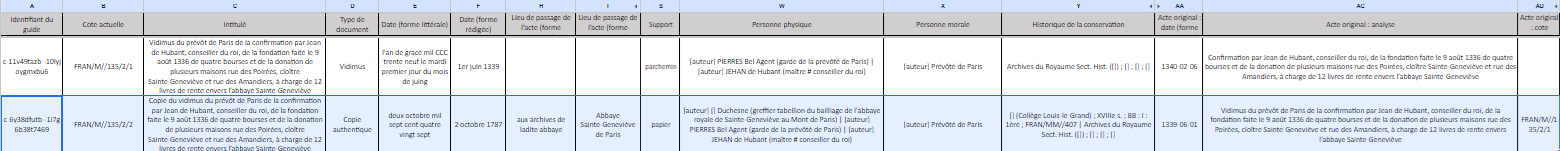
\includegraphics[width=1.14\linewidth]{images/ligne tableau.png}
    \caption{Ligne 1 et 2 du tableau de dépouillement du collège de Hubant.}
    \label{fig:tableau-depouillement-hubant}
\end{figure}
\begin{figure}[!h]
    \centering
    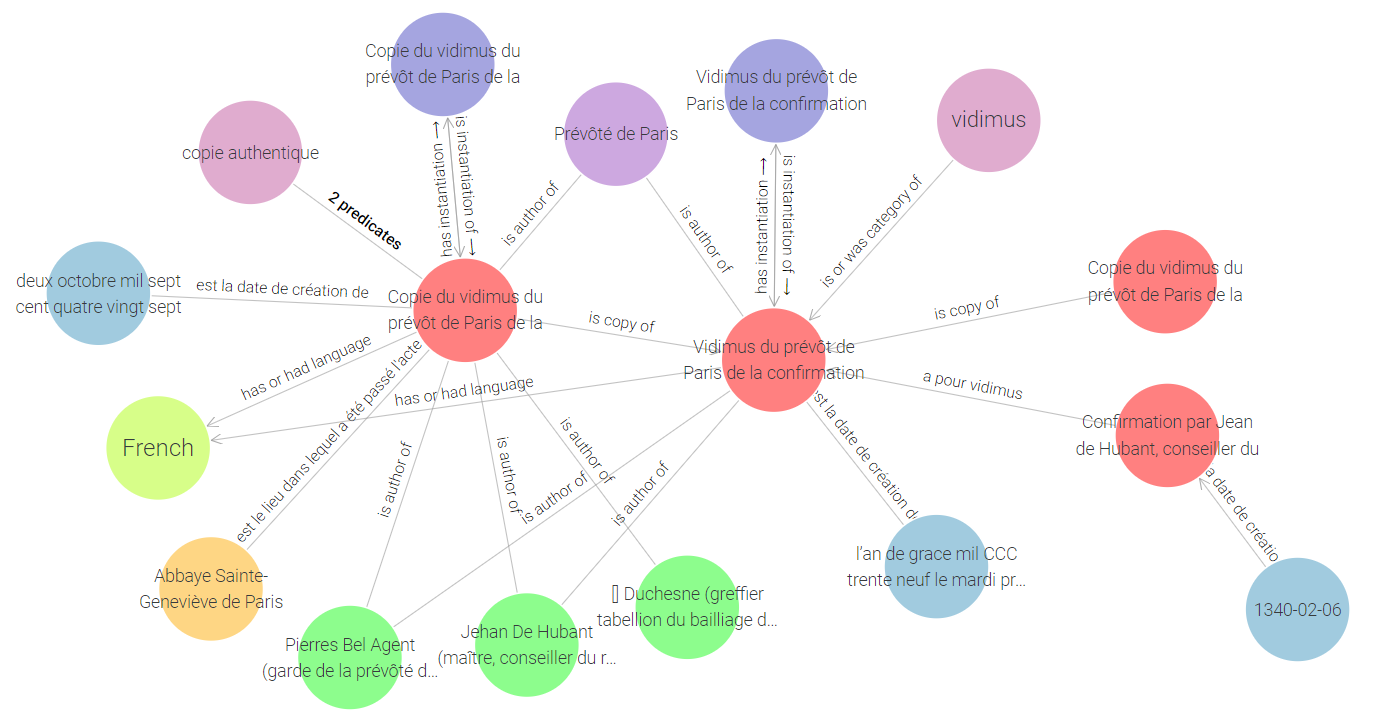
\includegraphics[width=0.9\linewidth]{images/visiualisation graphe hubant.png}
    \caption{Visualisation en graphe, de ces mêmes lignes transformées en RDF, centrée sur les RecordResource.}
    \label{fig:graphe-hubant}
\end{figure}
\subsection{SPARQL}
La seconde méthode consiste à utiliser l'éditeur de requête SPARQL. SPARQL (SPARQL Protocol and RDF Query Language) est un langage de requête spécifiquement conçu pour interroger les données RDF. Il offre une syntaxe expressive et puissante, permettant de formuler des requêtes complexes pour extraire des informations précises et pertinentes. De plus, il permet d'effectuer des requêtes distribuées, ce qui signifie qu'il peut interroger des sources multiples réparties dans le Web de données et ainsi permettre leur agrégation. Pour faciliter l'écriture des requêtes, SPARQL permet la déclaration de préfixes\footnote{Pour RiC-O ce préfixe (qui est déclaré dans l'ontologie) est \textbf{rico}, pour l'ontologie ORESM c'est \textbf{oresm-onto}.} qui remplacent la partie invariante des URIs\footnote{La partie invariante des URIs des composants de RiC-O est <https://www.ica.org/standards/RiC/ontology\#>.} d'une ontologie.
\begin{figure}[!h]
    \centering
    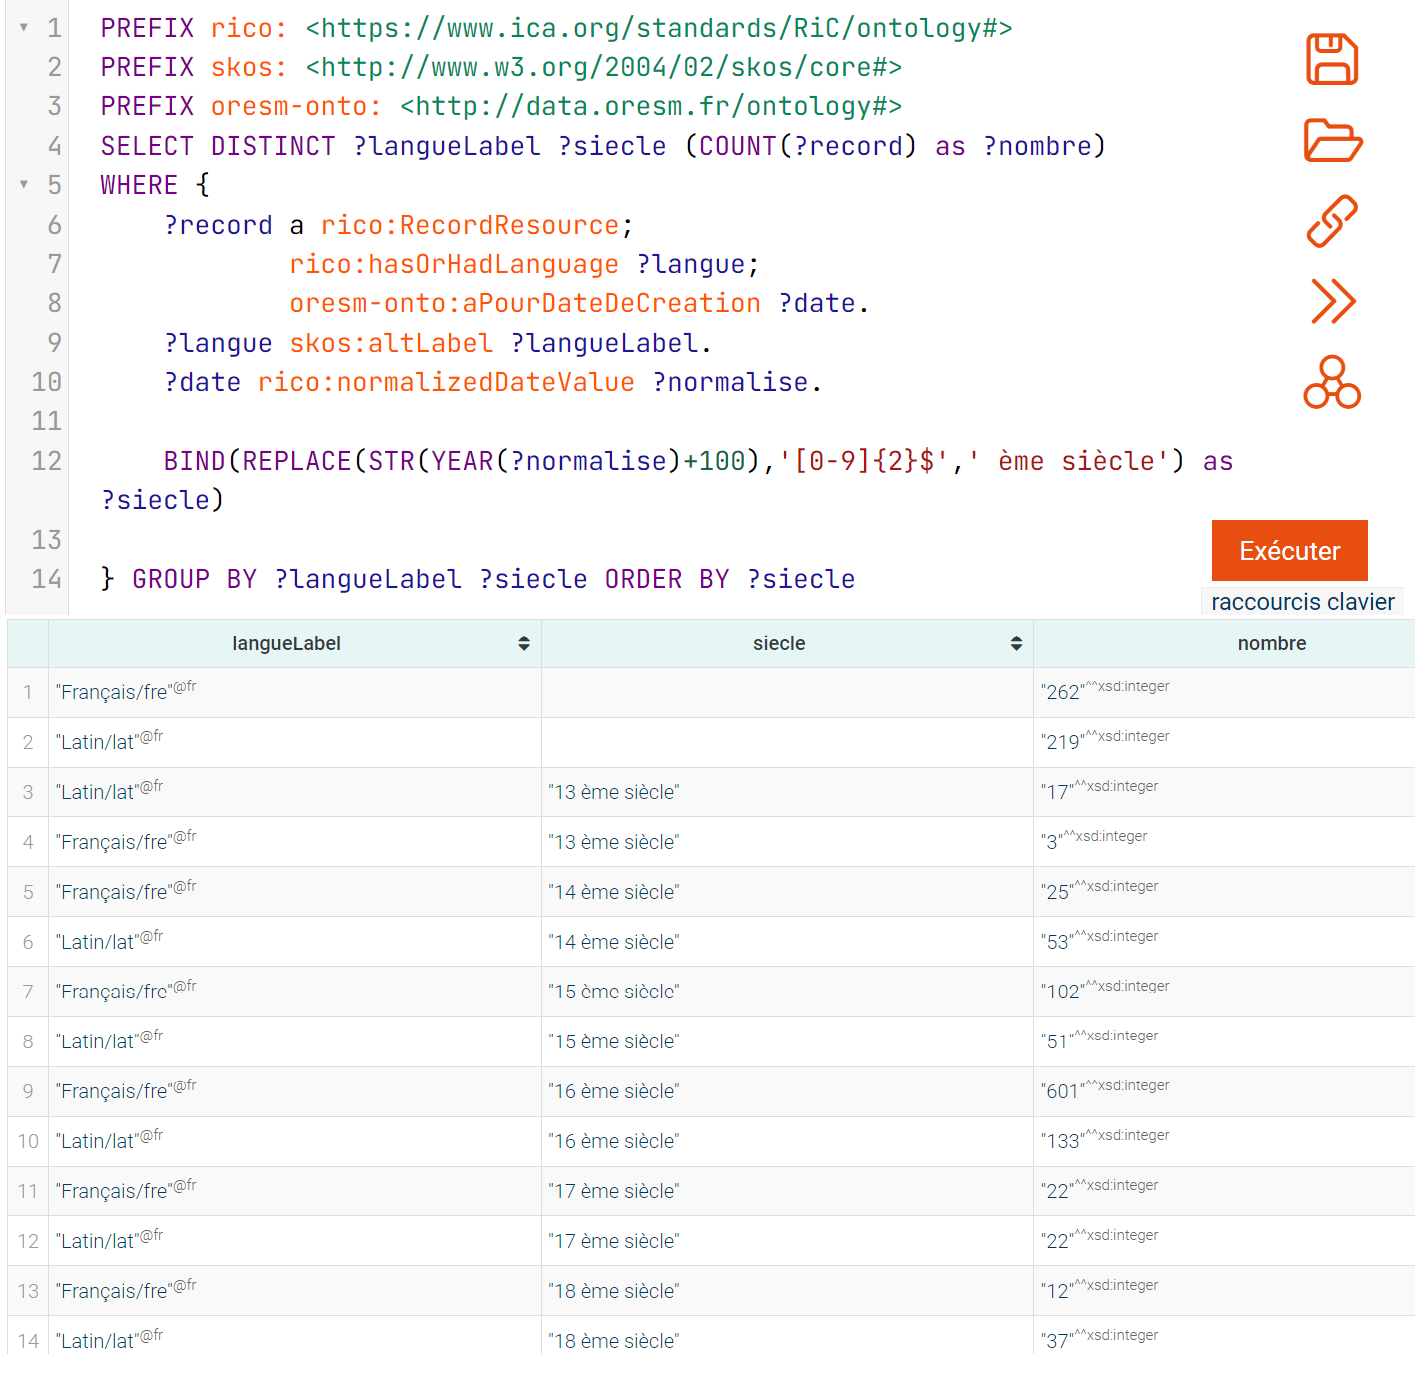
\includegraphics[width=0.95 \linewidth]{images/requete sparl langue resultat.png}
    \caption{Un exemple de requête SPARQL dans l'interface GraphDB et le résultat associé.}
    \label{fig:sparql_requete}
\end{figure}

Dans la requête d'exemple ci-dessus on opère une recherche sur les données. C'est le rôle du mot clé \textbf{SELECT}. SPARQL fonctionne en utilisant des variables, chaque variable peut être sujet, prédicat et/ou objet d'un triplet. Les résultats contiennent les valeurs que les variables contiennent quand l'ensemble des triplets dans la clause \textbf{WHERE} sont possibles. On peut également appliquer un traitement sur les données littérales, comme, dans l'exemple, avec des expressions régulières ou des opérations mathématiques, et on peut par ailleurs grouper les résultats. La requête d'exemple compte les documents d'archives par siècle et par langue. Ainsi on peut s'apercevoir qu'aux \textsc{XIII}\ieme{} et \textsc{XIV}\ieme{} siècle le latin domine dans les actes avant de se faire largement dépasser au \textsc{XV}\ieme{} et \textsc{XVI}\ieme{} siècle avec un rapport de un pour six. Certaines pièces sont bilingues ou n'ont pas de date sous forme normalisée, ce qui explique que le nombre total de pièces ne soit pas égal au nombre de pièces dépouillées (1441). Les pièces au-delà du \textsc{XVI}\ieme{}  siècle sont des copies de pièces beaucoup plus anciennes ce qui peut expliquer la prédominance du latin. C'est très puissant et on peut étendre ces requêtes avec d'autres conditions, des filtres, des unions etc. Une fois qu'on maîtrise bien le modèle et le langage SPARQL on peut faire beaucoup de choses et extraire des informations pertinentes.
\par
Mais SPARQL ne se limite pas à la lecture de données, on peut également insérer des données et même raisonner à partir de celles-ci pour ajouter de nouveaux triplets.\footnote{Lien de la spécification du W3C concernant SPARQL Update. \href{https://www.w3.org/TR/sparql11-update/}{https://www.w3.org/TR/sparql11-update/}} C'est un moyen parfait de créer de nouvelles assertions (nouveaux triplets) à partir de ceux déjà produits par le script de transformation et lors de l'import des données dans la base de graphe. Par exemple, les liens entre les personnes et les lieux, fondamentaux dans les enjeux du projet mais laissés de côté par le script. Il est aisé avec SPARQL d'ajouter des triplets. Prenons le cas d'un acte qui a un lieu de passage ; si cet acte a un rédacteur il est évident que le rédacteur de l'acte s'est trouvé un jour au lieu de passage. C'est la logique de la requête ci-dessous. La logique est claire, la rédaction rapide et le résultat efficace puisqu'on crée 225 nouveaux triplets en exécutant cette requête. Mais, comme nous l'avons déjà dit, ceci est aisé lorsqu'on connaît très bien à la fois SPARQL et le modèle de données, faute de quoi il est beaucoup plus difficile d'employer une telle méthode. Nous avons, en annexe de ce mémoire, mis une courte liste de requêtes SPARQL utilisées au cours du stage.\ref{sparql}
\begin{figure}[!h]
    \centering
    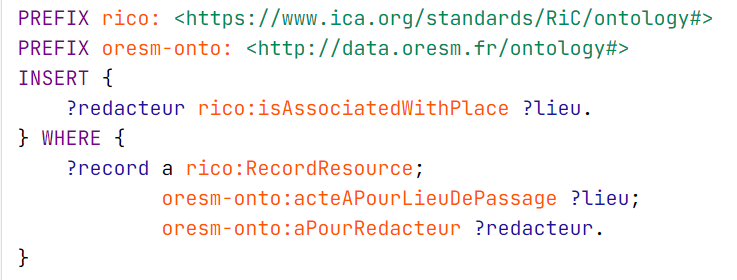
\includegraphics[width=0.9\linewidth]{images/insert redacteur.png}
    \caption{Requête SPARQL qui insère de nouveaux triplets dans le graphe en raisonnant sur le rédacteur et le lieu de passage d'un acte.}
    \label{fig:insert-redacteur}
\end{figure}
\chapter{Une interface de recherche adaptée}
Une fois que les données RDF produites sont chargées dans une base de graphes et rendues exploitables, il convient de les doter d'une interface de recherche pour ses futurs utilisateurs. Proposer uniquement l'éditeur de requêtes SPARQL brut, comme l'offre n'importe quel SPARQL end point, ne suffit pas : la grande majorité des utilisateurs finaux de données historiques ou archivistiques ne connaissent bien évidemment ni SPARQL ni l'ontologie de référence. En outre, exploiter véritablement un graphe, qui relie des entités appartenant à un nombre significatif de classes distinctes, par un nombre significatif de relations différentes, ne peut pas se faire par des biais classiques tel qu'un formulaire de recherche avancée. Il est nécessaire de trouver une solution permettant à l'utilisateur d'explorer ce graphe à sa guise. Dans le temps limité qui nous était imparti, nous avons choisi d'utiliser l'outil Sparnatural.
\begin{figure}[h]
    \centering
    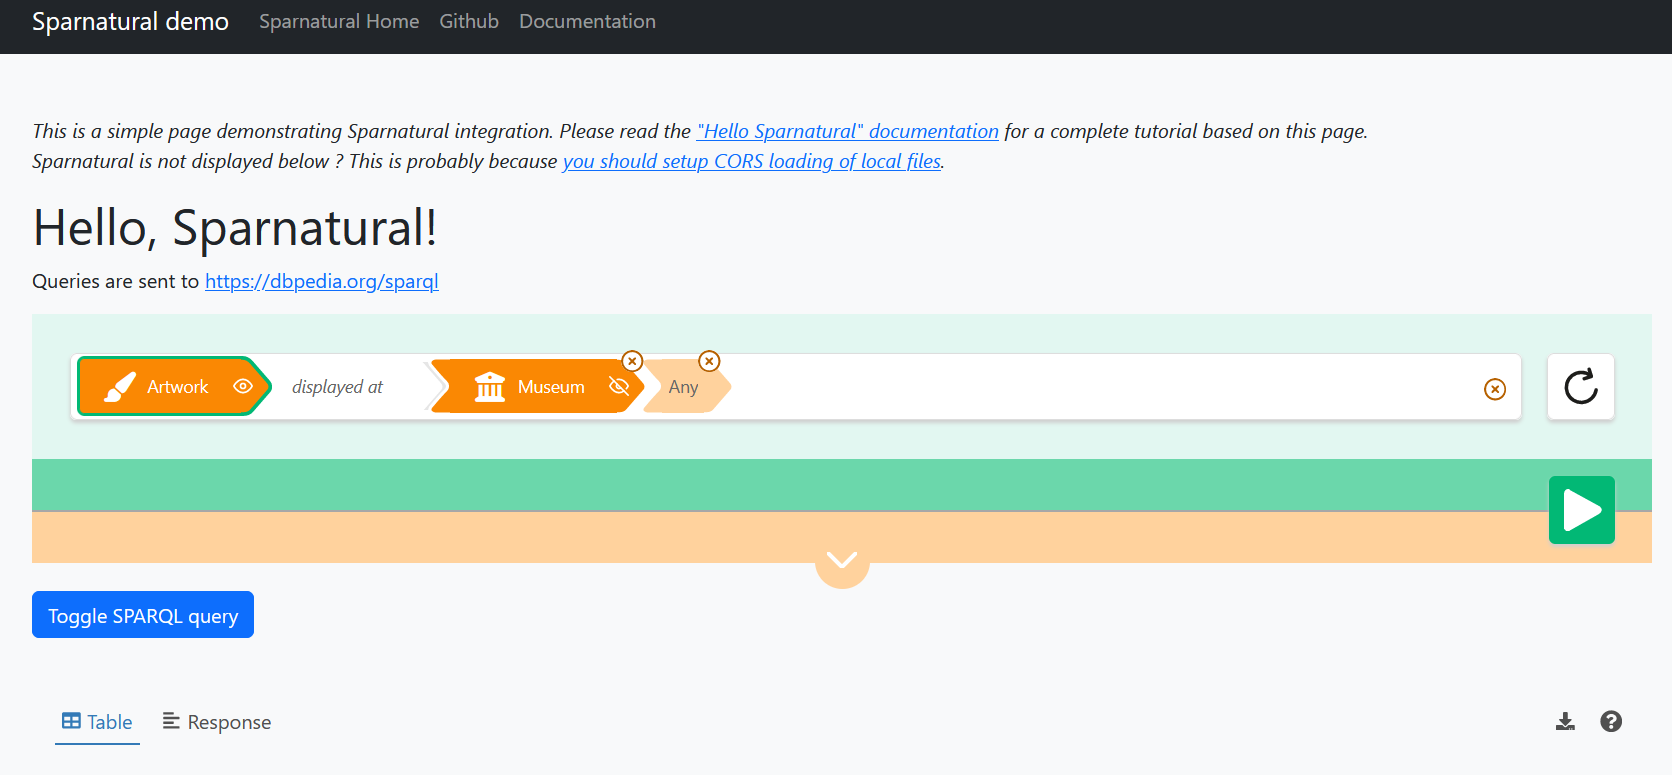
\includegraphics[width=1\linewidth]{images/hello sparnatural.png}
    \caption{L'exemple de la configuration classique de l'outil Sparnatural. Ici la requête interroge la base de données DB Pedia sur les oeuvres d'arts qui sont affichées dans n'importe quel musée.}
    \label{fig:hello-sparnatural}
\end{figure}
\section{La solution Sparnatural}
\subsection{Une interface sur mesure}
Sparnatural est un éditeur visuel open source et gratuit de requêtes SPARQL. Développé en JavaScript par 
la société Sparna, il permet à l'utilisateur de construire visuellement un questionnaire qui sera automatiquement traduit en requête SPARQL par l'outil. L'outil a d'abord été développé en 2018 par Sparna pour pouvoir doter le portail OpenArchaeo d'une interface web de recherche. Ses fonctionnalités, son design et sa documentation ont ensuite été fortement améliorés en 2021-2022, dans le cadre d'un projet associant la BnF, le ministère de la Culture et les Archives nationales (via le Lab qui a porté ce projet), qui a également permis à la BnF \footnote{Voici le lien du démonstrateur de la BNF : \href{https://data.bnf.fr/sparnatural/}{https://data.bnf.fr/sparnatural/}}et aux Archives nationales, en juin 2022, de mettre en ligne deux démonstrateurs. Le démonstrateur des Archives nationales a été réalisé par le Lab en collaboration avec Sparna et propose aujourd'hui deux interfaces de recherche. Il va très probablement évoluer en 2024, en même temps que l'outil, dans le cadre d'une troisième phase. Voyant les bons résultats ainsi obtenus pour des données RDF/RiC-O, l'équipe projet du portail FranceArchives a décidé de sémantiser les métadonnées du portail conformément à RiC-O 0.2 et de les rendre interrogeables via une interface utilisant également Sparnatural, publiée en septembre 2023. Compte tenu de ces précédentes expériences sur des projets d'envergure et des qualités de l'outil, il était logique d'envisager de l'utiliser également pour le futur portail ORESM. Nous avons pu avoir accès à une documentation avant sa publication. Cette documentation est très bien renseignée, une partie de celle-ci explique pas à pas la configuration d'une interface basique, et une autre montre l'ensemble des possibilités en configurant l'outil à l'aide d'une ontologie OWL. Il est à noter que les résultats des requêtes peuvent s'exporter au format CSV. Pour la réalisation d'une première interface de recherche, pour les données RDF que nous avions produites, nous avons utilisé la version 8.5 de Sparnatural, publiée en juillet dernier, et nous sommes partis de la configuration réalisée par Florence Clavaud pour la preuve de concept initiale.
\par
L'outil permet d'envoyer des requêtes à un Sparql Endpoint et d'afficher les résultats comme dans n'importe quel éditeur de requête SPARQL. La différence réside dans l'élaboration d'une interface qui représente les triplets interrogés d'une manière visuelle. On clique sur des boutons pour naviguer entre les possibilités définies par la configuration de l'interface. De cette manière l'utilisateur n'est pas obligé de connaître le modèle de données, mais il doit tout de même élaborer sa recherche d'une manière conceptuelle : quelles sont les entités qu'il recherche ? Quelles sont les caractéristiques ou les relations de ces entités sur lesquelles il veut effectuer sa recherche ? La conception d'une requête reste à appréhender, mais on a éliminé le problème de la connaissance de l'ontologie et du langage SPARQL. 
\par
Pourtant Sparnatural est agnostique, c'est à dire qu'il est utilisable pour n'importe quel jeu de données RDF conforme à n'importe quelle ontologie. C'est lors de sa configuration, qui peut notamment se faire via un fichier OWL\footnote{Le fichier OWL est le type de fichier utilisé pour construire une ontologie.}, qu'on définit quelles entités et quelles relations l'utilisateur final va pouvoir employer dans la construction de sa requête. Il s'agit finalement de \textit{"spécifier un modèle ontologique pour la recherche et ses correspondances avec les classes et propriétés de l’ontologie métier"}.\footnote{Citation tirée de la documentation du projet de démonstrateur des AN : \href{https://sparna-git.github.io/sparnatural-demonstrateur-an/presentation-fr.html\#design}{https://sparna-git.github.io/sparnatural-demonstrateur-an/presentation-fr.html\#design}}


\subsection{Modélisation de l'interface}
Nous avons donc choisi cette méthode de configuration par une ontologie. Il y a d'abord eu un travail de modélisation à faire. Puisque l'idée initiale de la preuve de concept était de traiter absolument toutes les données contenues dans les fichiers Excel de dépouillements, alors il fallait pouvoir toutes les interroger pour permettre une relecture. Nous avons réalisé une modélisation avant de nous lancer dans la configuration, des critères de requête nécessaires pour interroger l'ensemble de nos données (voir le schéma de modélisation ci-dessous). Dans cette modélisation, on voit que la majorité des types d'information que nous avons sont liés à la pièce d'archives. Tout passe par la ressource archivistique qui reste la composante essentielle de la majorité de nos triplets. Avec cette configuration plus besoin de différencier, comme dans le modèle RiC-O, le RecordResource et l'Instantiation, c'est une notion qui est utile en terme de gestion de données mais ne servira à rien pour le chercheur utilisateur. Certains choix ont été faits aussi concernant la question du sceau. Nous avons décidé de créer un critère particulier pour les relations entre une ressource archivistique et son sceau. Utiliser directement, comme c'était exprimé dans les tableaux de dépouillements et l'ontologie ORESM, un critère sur les caractéristiques physiques aurait rendu la recherche malaisée. Nous avons beaucoup de granularités dans nos données, et dans un cas comme le nôtre il ne faut pas surcharger l'interface d'éléments au risque de perdre et décourager l'utilisateur mais il ne faut pas non plus trop limiter les possibilités de recherche pour les utilisateurs déterminés. Il faut chercher à \textit{" atteindre par ce biais un compromis raisonnable entre la complexité du modèle métier et la nécessité de produire une interface compréhensible et performante pour les utilisateurs"}\footnote{Citation tirée de la documentation du projet du démonstrateur des AN : \href{https://sparna-git.github.io/sparnatural-demonstrateur-an/presentation-fr.html\#design}{https://sparna-git.github.io/sparnatural-demonstrateur-an/presentation-fr.html\#design}}

\begin{figure}[h]
    \centering
    \includegraphics[width=1.1\linewidth]{images/sparnatural shéma.PNG}
    \caption{Modélisation du système de requête dans notre interface Sparnatural}
    \label{fig:shéma_sparnatural}
\end{figure}

\section{La configuration ORESM}
\subsection{Édition sur Protégé}
Puisque le fichier de configuration se base sur le langage OWL, il est possible de l'éditer avec le logiciel Protégé. La logique hiérarchique des classes importe peu, on les distingue en deux types, les classes représentant des types d'entités RDF, et associées à un ou plusieurs URI, et les classes qu'on appelle littérales qui permettent d'accéder aux Datatypes properties. La configuration de l'interface pour les classes nous a paru assez simple puisque nous disposions d'une bonne documentation, que nous connaissions nos données, l'ontologie ORESM et avions défini notre modèle de requêtes. On peut donner des attributs aux différentes classes, ils permettent d'afficher davantage d'informations à l'utilisateur. L'attribut \textit{tooltip} permet d'afficher un message de description lorsque le curseur est sur l'objet concerné. Il est également recommandé d'utiliser des icônes pour améliorer l'expérience utilisateur, pour ce faire il faut indiquer pour la valeur de l'attribut \textit{fontawesome icon code} le code associé à cette icône sur le site \href{https://fontawesome.com/}{Font Awesome}. On peut aussi spécifier l'ordre d'apparition des classes qui seront les premiers points d'entrée dans le graphe, avec l'attribut \textit{order}.
\begin{figure}[h]
    \centering
    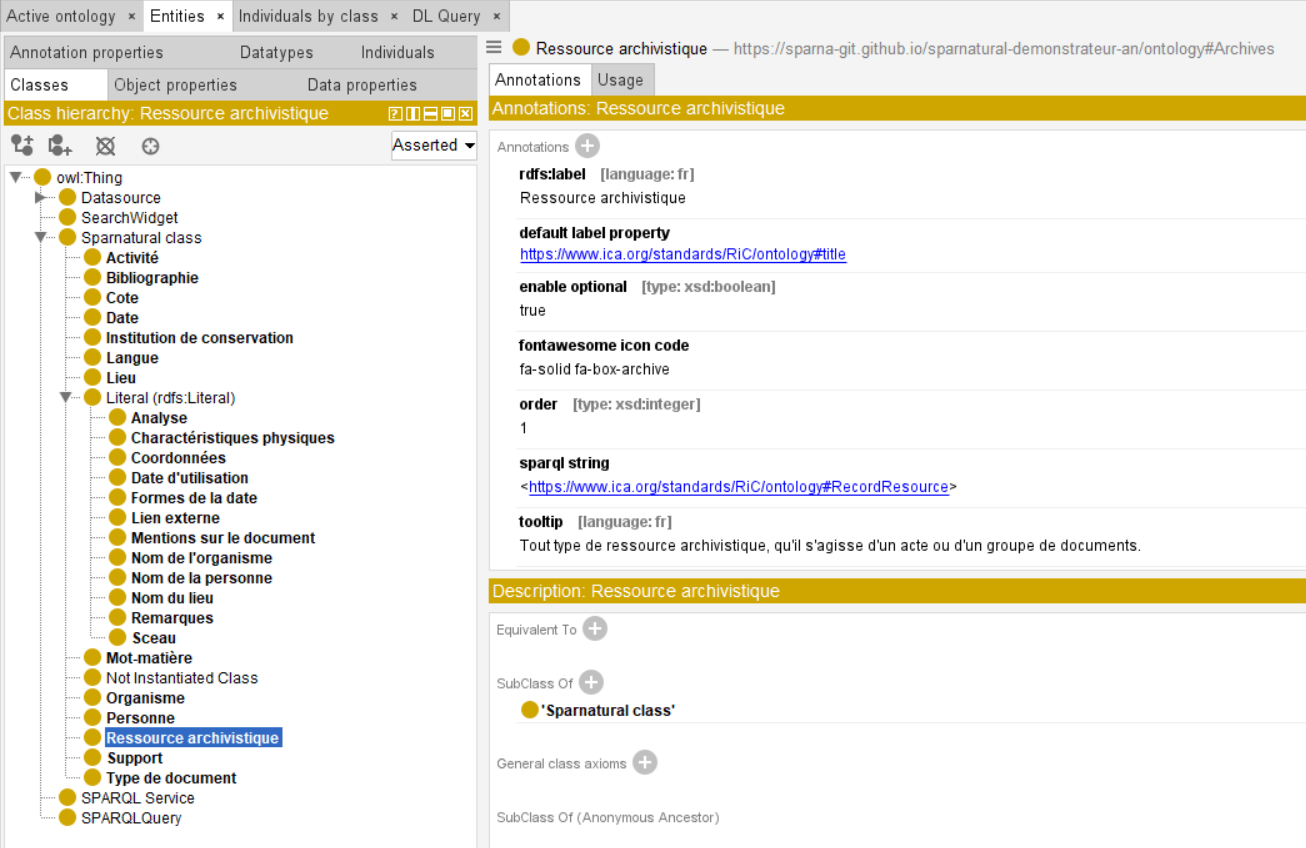
\includegraphics[width=0.9\linewidth]{images/classes sparnatural.png}
    \caption{Capture d'écran des classes créées pour la configuration de l'interface Sparnatural avec les attributs des Ressources Archivistiques.}
    \label{fig:classes-sparnatural}
\end{figure}

Pour ce qui est des relations, plusieurs catégories sont mises à disposition. Quand il s'agit d'une relation ayant pour cible une classe d'entités, un système de liste ou d'auto-complétion permet de viser une entité précise en parcourant les données avant même d'avoir exécuté la requête\footnote{Ces dispositifs permettent en général d'interroger la datatype property rdfs:label d'une instance de classe.}. Une liste est plus efficace pour un nombre restreint d'éléments, c'est l'inverse pour l'auto-complétion. Les autres liens, ceux visant des valeurs littérales peuvent être de plusieurs catégories ; en fonction de ces catégories l'interface proposera différentes manières de filtrer la valeur. On peut disposer d'une simple zone de saisie, d'un choix booléen, d'une carte pour sélectionner des coordonnées géographiques ou même d'un calendrier pour choisir un intervalle de date. Évidemment ces options servent à appliquer un filtre sur les données mais pour chacune d'entre elles on peut également décider d'accepter toutes les valeurs. Pour ce qui est de l'interprétation en SPARQL il faut remplir le champ \textbf{sparql string}\footnote{Voir ci dessous l'exemple de valeur qu'il peut prendre.}. 
\par
Prenons l'exemple qui concerne le lien \textbf{est conservé actuellement par}. On spécifie que cette relation part (on dit qu'elle a pour domaine)  de la "Ressource Archivistique" et cible (on dit qu'elle a pour portée) une "Institution de conservation", respectivement un rico:RecordResource et un rico:CorporateBody. Sparnatural utilise pour générer ses requêtes les possibilités offertes par SPARQL pour parcourir un graphe de manière concise. On indique simplement la relation en utilisant la syntaxe proposé par le W3C\footnote{\href{https://www.w3.org/TR/sparql11-query/\#propertypaths}{Lien des spécifications W3C concernant la syntaxe des Property Path}}. Sparnatural met également à disposition un éditeur de requête SPARQL. On peut donc voir l'équivalent en SPARQL des requêtes construites avec l'éditeur visuel. Les personnes connaissant le langage préféreront sans doute y saisir directement leurs requêtes puisque cela permettra davantage de possibilités mais il n'y a aucune assistance à la saisie (par exemple pas d'auto-complétion).

\begin{figure}[h]
    \centering
    \includegraphics[width=1\linewidth]{images/sparnatural est conservé.png}
    \caption{Valeur du champ sparql string qui contient une expression SPARQL utilisée pour la relation \textbf{est conservé actuellement par}.}
    \label{fig:lien-sparnatural-conserve}
\end{figure}
\begin{figure}[h]
    \centering
    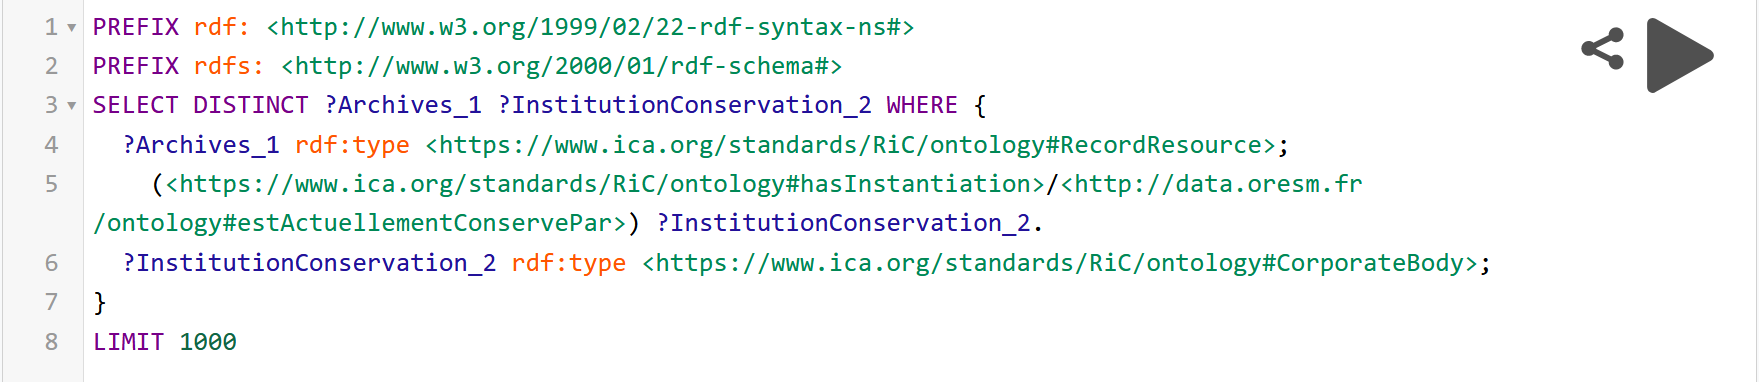
\includegraphics[width=1\linewidth]{images/equivalent sparql.png}
    \caption{Équivalent de cette relation dans l'éditeur de requête SPARQL.}
    \label{fig:lien-sparql-conserve}
\end{figure}

\subsection{Présentation de l'interface}
Finalement nous avons décidé de configurer deux interfaces, la première pour la recherche avancée, qui se base sur le modèle présenté plus tôt, et une autre de recherche simple. Celle-ci veut simuler une recherche plein texte avec l'outil Sparnatural ; ce n'est absolument pas une configuration définitive (tout comme celle avancée d'ailleurs). La recherche simple est présente pour voir si il était possible de faire ce type de recherche sur les données. La valeur écrite dans la zone de saisie est recherchée dans l'ensemble des rdfs:label de nos entités. C'est donc techniquement faisable mais il faudra revoir l'interface. Les réponses sont rapides, toujours en dessous de 0,5 seconde, ce qui était la principale inquiétude de cette recherche plein texte.\footnote{Pour ce type de recherche l'interface ORESM devrait pouvoir bénéficier en 2024 d'une évolution de Sparnatural qui irait en ce sens.} Voici quelques captures d'écran de l'interface utilisée.

\begin{figure}[!h]
    \centering
    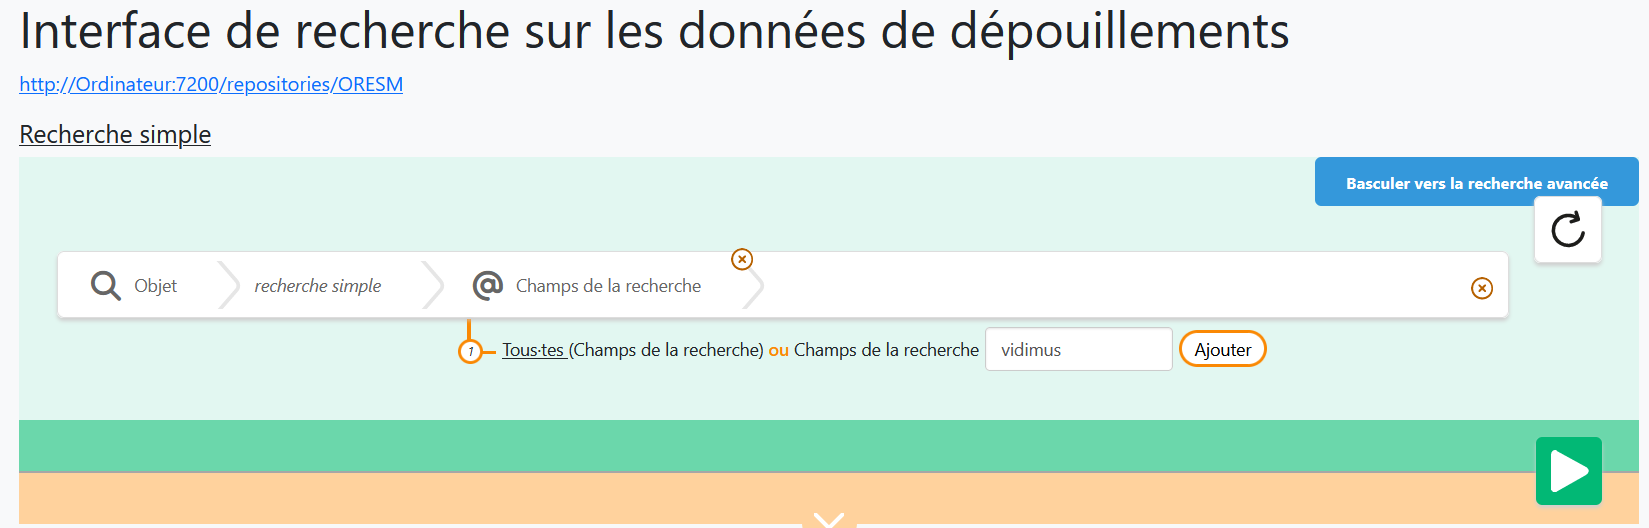
\includegraphics[width=1.1\linewidth]{images/recherche-simple.png}
    \caption{Interface de la recherche simple. On ne peut sélectionner qu'un unique élément.}
    \label{fig:recherche-simple}
\end{figure}
\begin{figure}[!ht]
    \centering
    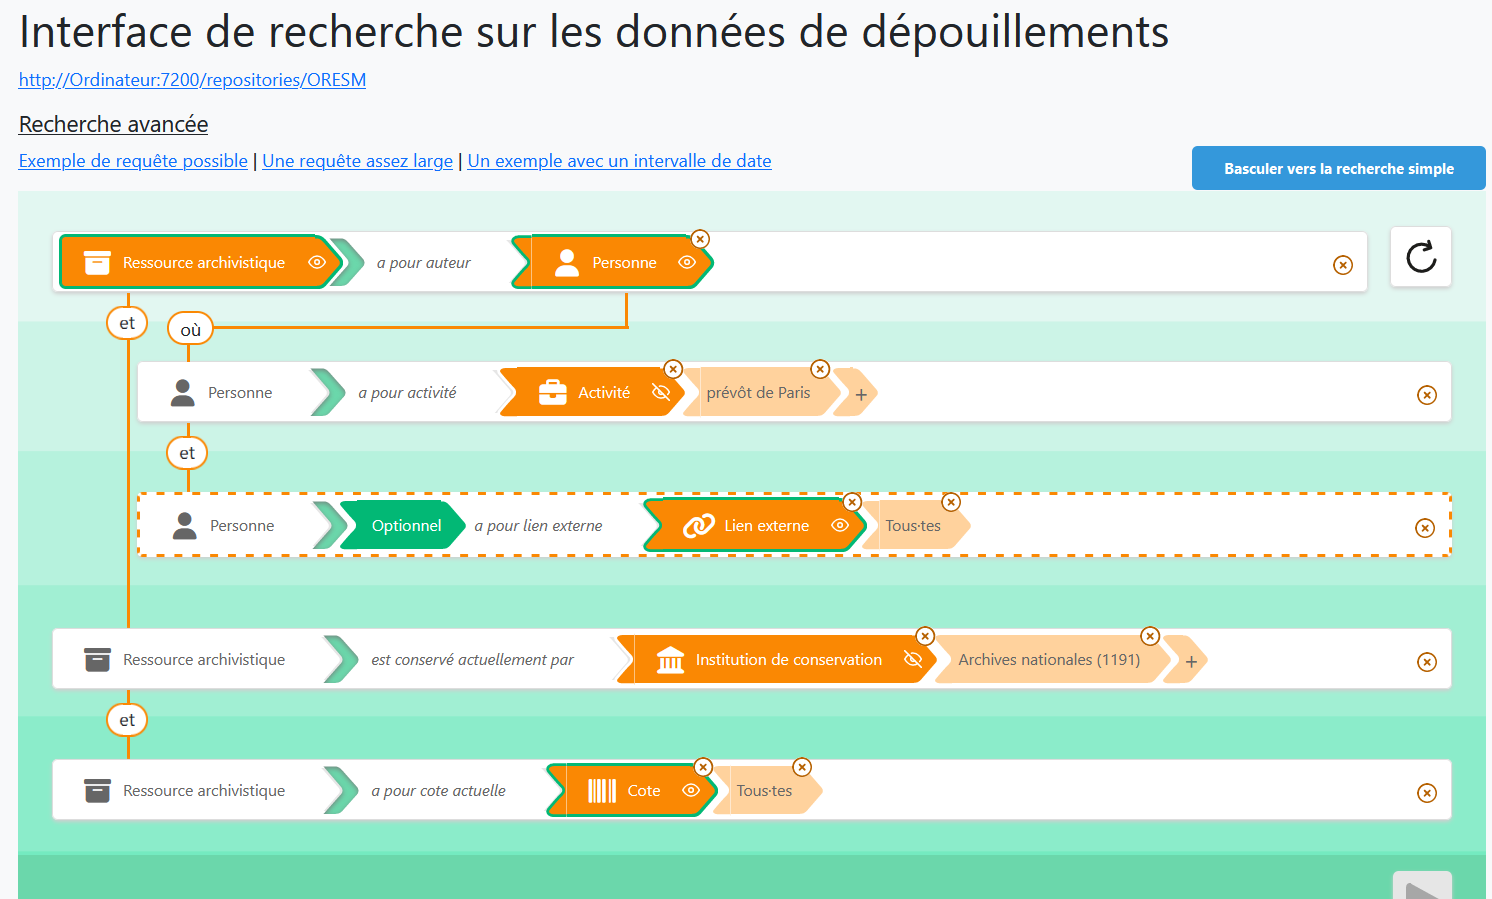
\includegraphics[width=1\linewidth]{images/interface-oresm-exemple.png}
    \caption{Exemple d'une requête avancée conçue à partir de l'interface Sparnatural.}
    \label{fig:recherche-avancée}
    \centering
    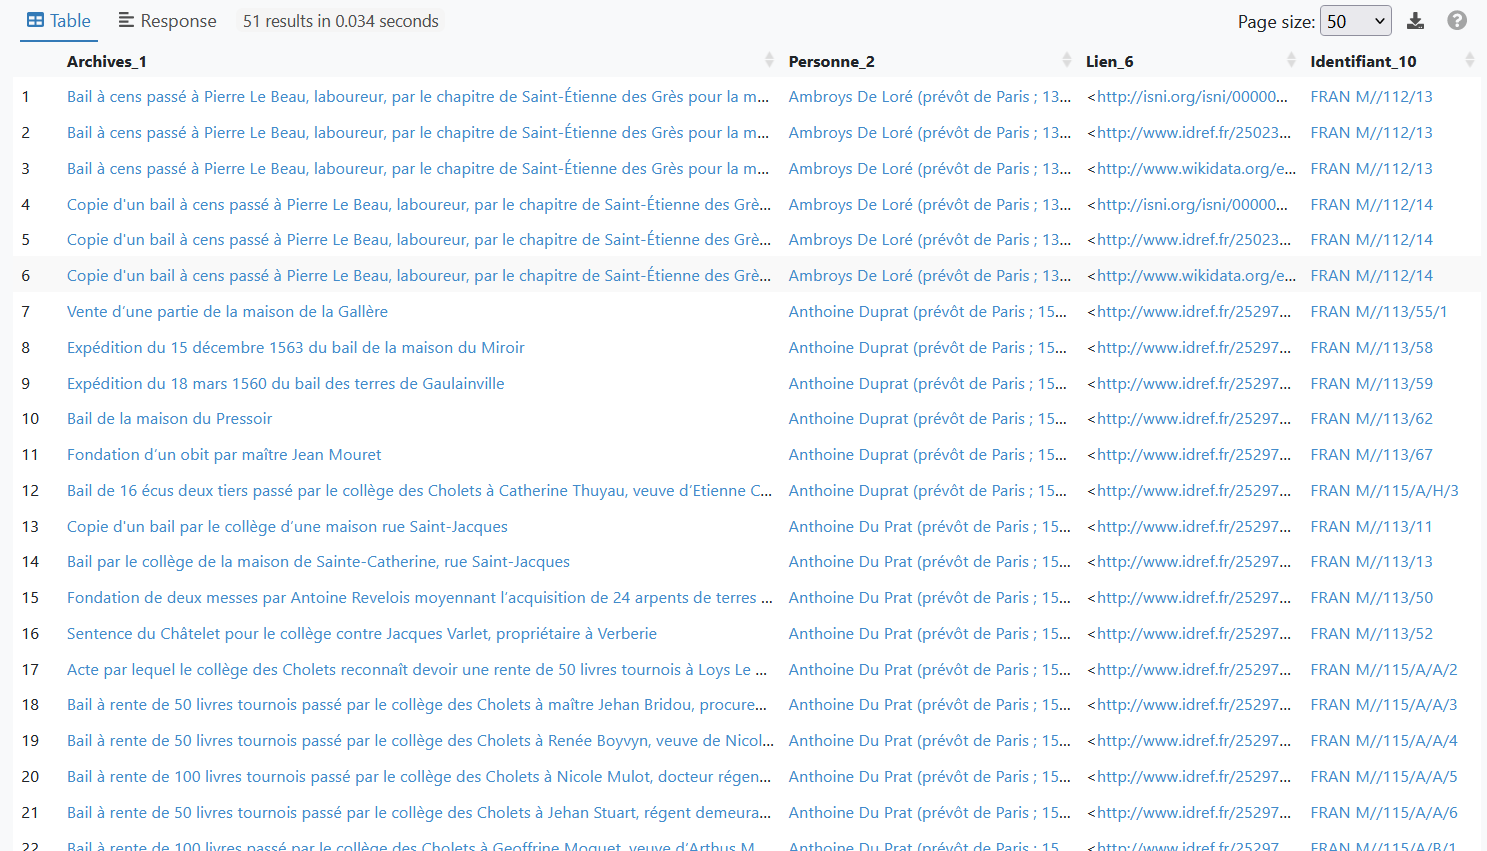
\includegraphics[width=1\linewidth]{images/resultat-requete-sparnatural.png}
    \caption{Le résultat de la requête. Les labels de chaque éléments sont affichés, ce sont des liens vers l'URI de l'entité.}
    \label{fig:resultat-sparnatural}
\end{figure}

\par
Il faut toutefois remettre les choses dans le contexte de notre stage, pour lequel nous ne disposions que d'un temps très limité. Cette interface a été avant tout réalisée pour prendre l'outil en main. Avec celui-ci nous avons testé notre modèle de données. Grâce à Sparnatural nous pouvons illustrer les possibilités offertes avant de lancer un recueil de besoins. Nous avions besoin d'un support suffisamment complet et développé à remettre aux chercheurs. Avec cette configuration temporaire ils auront une base pour faire des commentaires, émettre des envies et indiquer ce qui ne va pas. La base de donnée et l'interface ont été déployées par Sébastien Clément sur un serveur test de la BIS pour préparer cette étape. Il nous faut avoir en tête que notre travail devra répondre avant tout aux besoins des futurs utilisateurs du portail ORESM. L'ensemble de cette interface ne sera pas le résultat mis en ligne mais plutôt le moyen de faire éprouver l'ensemble de la preuve de concept réalisée dans le cadre de ce stage aux différents acteurs du projet.

\bookmarksetup{startatroot}
\chapter*{Bilan et perspectives d'évolution}
\addcontentsline{toc}{chapter}{Bilan et perspectives d'évolution}
Finalement que pouvons nous tirer des réalisations de ce stage ? Tout d'abord la faisabilité de la chose. La granularité de nos données et leur complexité étaient les difficultés principales. Aucun autre projet utilisant RiC-O n'avait amené une description aussi précise d'archives médiévales, avec toutes les spécificités que cela implique. Il a fallu, pour opérer la transformation des données en fichiers tabulaires en un seul graphe de connaissance, faire un travail de réflexion sur leur sémantisation tout en prenant en compte les objectifs du projet. Il en ressort un processus de construction et de transformation des métadonnées clairement défini. Les méthodes employées sont documentées. L'exploitation bien que très partielle démontre de grandes possibilités. C'est encourageant pour la suite. Le projet s'inscrit dans la transition qui va arriver dans le monde des archives vers de nouvelles normes de description des métadonnées et peut s'enorgueillir d'être à la pointe en termes d'actualités technologiques. Mais il reste encore de nombreux chantiers avant d'arriver à un résultat publiable.
\par
Étant donné le temps disponible pendant notre stage tout ne pouvait pas être traité. Il a fallu mettre de côté certains aspects du projet, pour pouvoir produire à temps un résultat exploitable. A plusieurs reprises au cours du stage nous nous sommes fait la réflexion qu'avec un tel niveau de description nous pouvions passer des mois et des mois à parfaire nos données, à continuellement chercher à améliorer le modèle ou la transformation. Pourtant la meilleure manière pour progresser dans un projet est d'avancer, puis de revenir, si le besoin se fait sentir, sur une tâche antérieure, avec l'expérience acquise. Avec ce procédé nous avons une vision plus globale, ce qui éclaire la prise de décision. Nul doute que les éléments acquis à travers ce stage serviront de support aux différentes évolutions du projet.
\par
Par exemple, comme nous l'avons déjà évoqué, les remarques saisies dans les tableaux de dépouillement sont de nature très diverse. Ce qui est pratique et intellectuellement satisfaisant, lors d'une étape de saisie dans un tableau, n'est pas exploitable lorsqu'on s'attache à produire un graphe de haute qualité dans le cadre d'un projet de recherche. En partant de ce postulat, et avec le recrutement de nouveaux archivistes pour poursuivre les dépouillements, nous avons émis des recommandations afin de faciliter la transformation en RDF. Pour continuer sur cet exemple, il a été recommandé de typer les remarques\footnote{Voir le tableau rempli à cette occasion \href{https://github.com/Florian-Langele/Memoire-de-stage-TNAH/blob/main/Livrables/Typologie\%20des\%20remarques.xlsx}{Livrables/Typologie des remarques.xlsx}} par rapport à l'entité RiC-O auxquelles elles se rapportent. De manière plus générale, les données traitées lors du stage proviennent d'une seule archiviste, et évidemment en tant que humain celle-ci avait sa manière personnelle de saisir les données. Et même si elle suivait une méthodologie, elle avait sa logique propre sur laquelle se base le script de transformation. Avec l'arrivée de nouvelles personnes sur les dépouillements, les prochains mois permettront d'ajuster en parallèle, si nécessaire,  la méthodologie de saisie et le script de conversion.
\par
Il reste encore un travail à faire pour gérer la normalisation des noms de personnes et la réconciliation des entités nommées. Un point majeur du sujet prosopographique repose sur l'incertitude qu'on a concernant une personne apparaissant sur deux actes différents. Quand la personne occupe un rang important on sait beaucoup de choses sur elle et on peut s'y retrouver. Mais sur la majorité des personnes citées dans nos archives on ne sait rien de plus que ce que nous avons pu tirer des documents. D'autant plus que la période étudiée, l'époque médiévale, voit des formes de noms très variées. Parfois une même personne peut être identifiée dans plusieurs documents sous un même nom mais avec une graphie différente. Il est donc souvent impossible d'affirmer une identité entre deux personnes; on peut seulement spécifier une probabilité et tenter de quantifier le niveau d'incertitude qui en résulte. C'est l'objectif de la base de données Studium Parisiense de réunir toutes les informations sur les personnes liées à l'Université de Paris au Moyen Âge. La sémantisation de cette base et, plus largement, la réalisation d'un référentiel des personnes permettant d'opérer ces réconciliations en fonction de critères précis et de consigner un niveau d'incertitude, sont prévues dans le cadre du projet ORESM. Il conviendra de faire en sorte que ce référentiel et le graphe de connaissance que nous avons commencé à produire soient liés, voire échangent des données.
 
\par
Il faut également réfléchir à l'intégration de nos données dans l'inventaire virtuel. Une des pistes possibles serait d'utiliser RiC-O Converter sur les fichiers EAD ; cependant rien n'est décidé à ce stade. Une chose est certaine : il faudra intégrer au graphe les données qui concernent les ensembles d'archives dans lesquels les pièces décrites s'inscrivaient au Moyen Âge. L'expérience acquise sera essentielle pour assurer une fusion propre et efficace de ces données.
\par
Pour ce qui est de la préparation de l'interface Sparnatural, la configuration actuelle a été déployée sur un serveur interne à la BIS pour préparer une relecture et un recueil des besoins. Beaucoup d'autres choses restent à faire en ce qui concerne l'interface : Sparnatural est un des dispositifs, il faudra en mettre en place d'autres. Notamment pour afficher les données relatives à une unique entité. Ce stage n'était qu'une étape.

\chapter*{Conclusion}
\addcontentsline{toc}{chapter}{Conclusion}
Ce mémoire rend compte des différents processus conçus pour exploiter efficacement des données archivistiques précises. Au départ de ce stage, nous disposions de plusieurs fichiers tabulaires, homogènement structurés et décrivant des archives médiévales. En utilisant les bases, posées par la preuve de concept de Florence Clavaud, nous avons réalisé un traitement sur les données extraites de ces fichiers. Avec un unique script, nous avons automatisé la sémantisation de ces données au format RDF/XML. Ce script se base sur le \textit{data mapping}, qui fait correspondre chacun des champs définis par la méthodologie de dépouillement avec un élément de l'ontologie ORESM, qui étend l'ontologie RiC-O. Un début d'interface a été mis en place, en utilisant l'outil Sparnatural, pour permettre l'interrogation des données à l'aide d'un constructeur de requête visuel. Bien que les réalisations de ce stage soient concluantes, beaucoup de choses restes à faire avant leurs exploitations complètes pour répondre aux enjeux scientifiques du projet.
\par
Participer au projet ORESM a été particulièrement formateur. Par les différents interlocuteurs que ce projet réunit, il a permis d'en apprendre davantage sur plusieurs milieux, notamment le monde de la recherche, des bibliothèques et des archives, et évidemment sur le dialogue nécessaire pour faire travailler conjointement les différents acteurs issus de ces milieux. Quelques années vont encore être nécessaires pour réaliser l'ensemble des objectifs prévus, mais nul doute qu'une fois la plateforme ORESM achevée celle-ci aura une place particulière pour la recherche sur l'ancienne université de Paris et la valorisation de son patrimoine.

\appendix

\chapter{Méthodologie des dépouillements}
\label{methodologie}
\begin{figure}[!h]
    \centering
    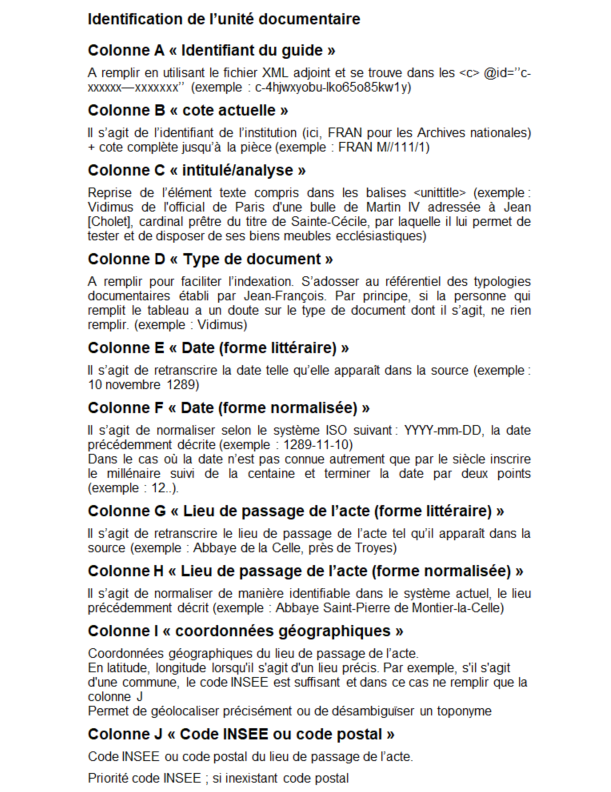
\includegraphics[width=0.75\linewidth]{annexes/methodologie1.png}
\end{figure}
\begin{figure}[!h]
    \centering
    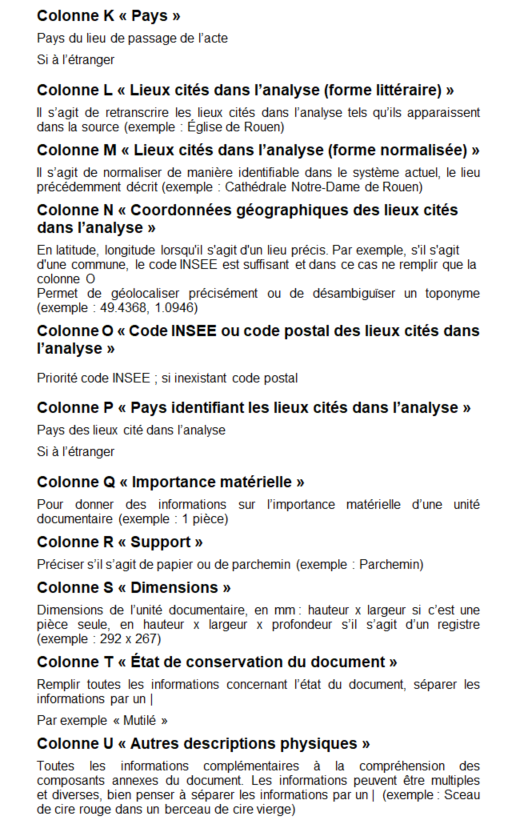
\includegraphics[width=0.85\linewidth]{annexes/methodologie2.png}
\end{figure}
\begin{figure}[!h]
    \centering
    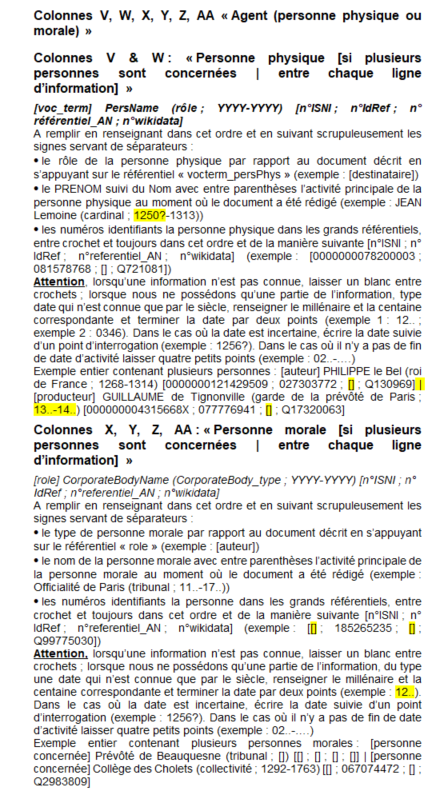
\includegraphics[width=0.85\linewidth]{annexes/methodologie3.png}
\end{figure}
\begin{figure}[!h]
    \centering
    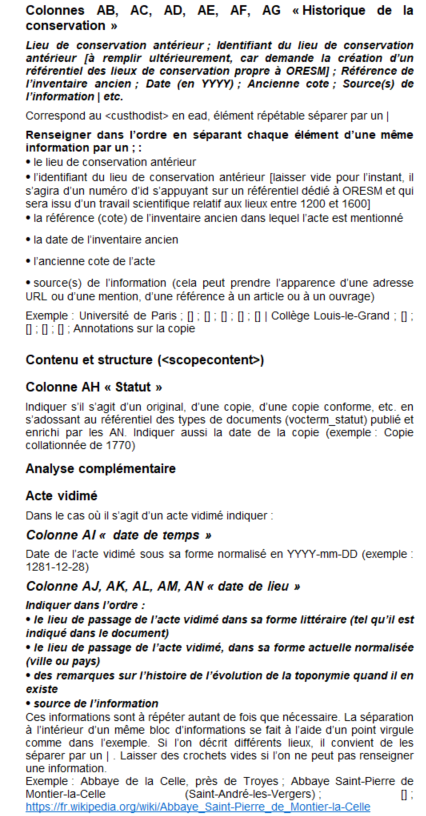
\includegraphics[width=0.85\linewidth]{annexes/methodologie4.png}
\end{figure}
\begin{figure}[!h]
    \centering
    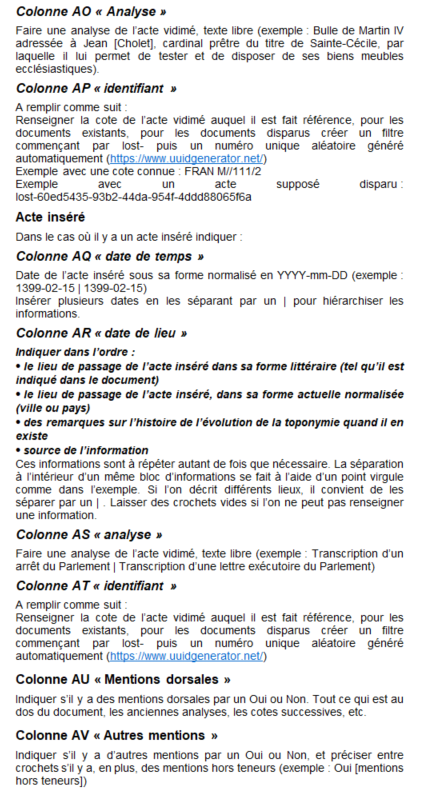
\includegraphics[width=0.85\linewidth]{annexes/methodologie5.png}
\end{figure}
\begin{figure}[!h]
    \centering
    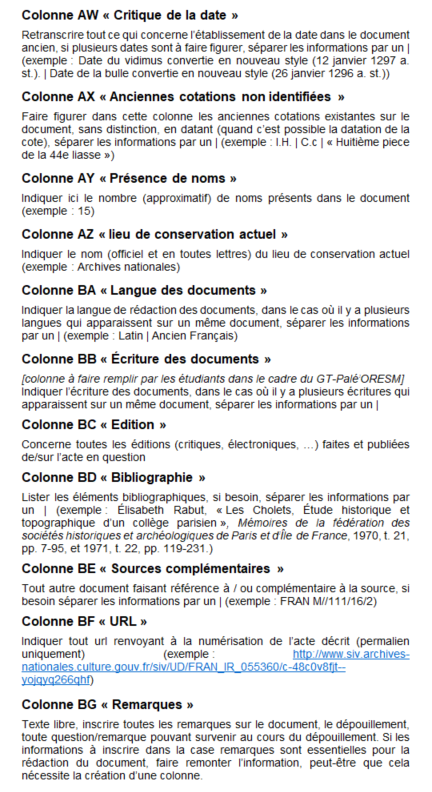
\includegraphics[width=0.85\linewidth]{annexes/methodologie6.png}
\end{figure}

\chapter{Tableau de mapping}
\label{mapping}
\begin{figure}[!h]
    \centering
    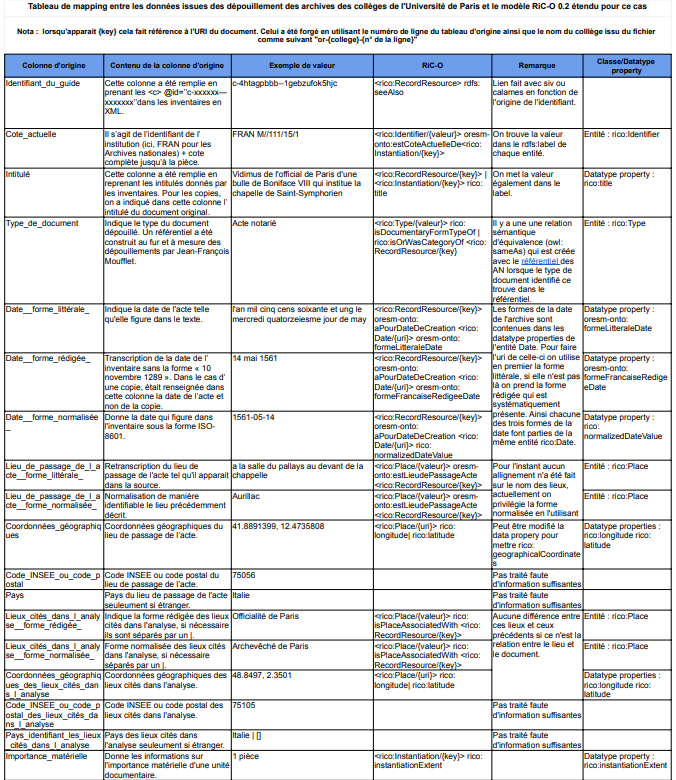
\includegraphics[height=1\linewidth]{annexes/mapping1.png}
\end{figure}
\begin{figure}[!h]
    \centering
    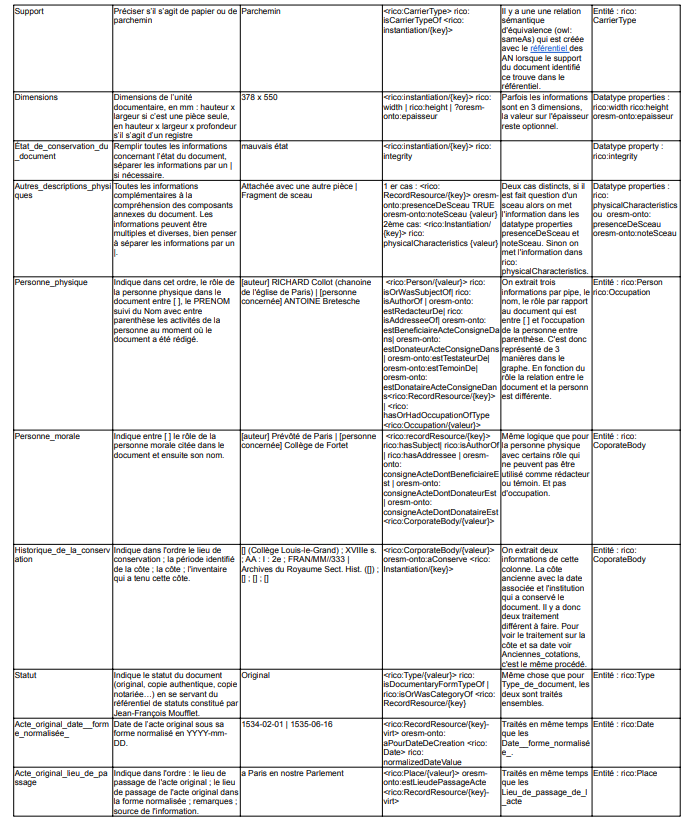
\includegraphics[width=1\linewidth]{annexes/mapping2.png}
\end{figure}
\begin{figure}[!h]
    \centering
    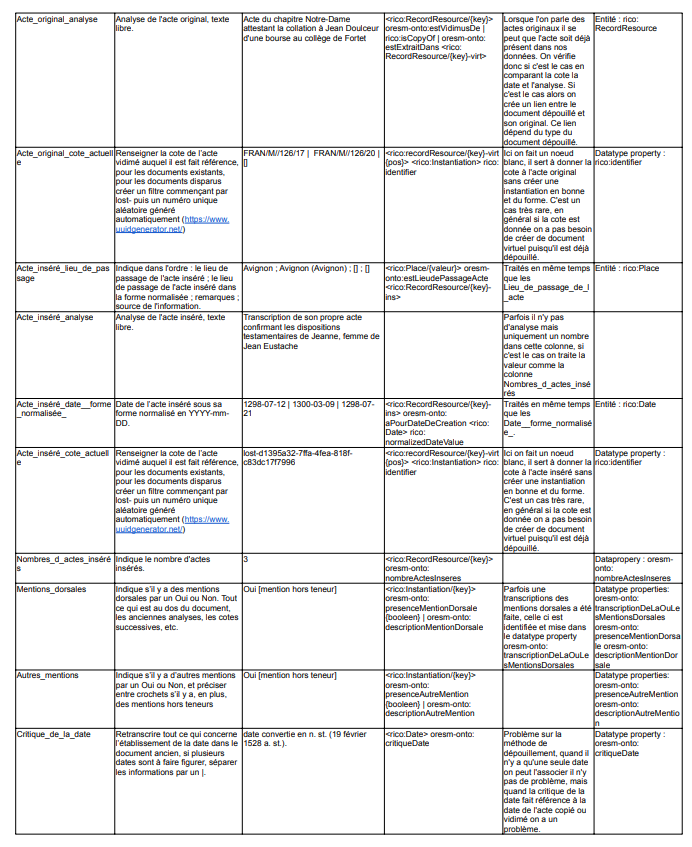
\includegraphics[width=1\linewidth]{annexes/mapping3.png}
\end{figure}
\begin{figure}[!h]
    \centering
    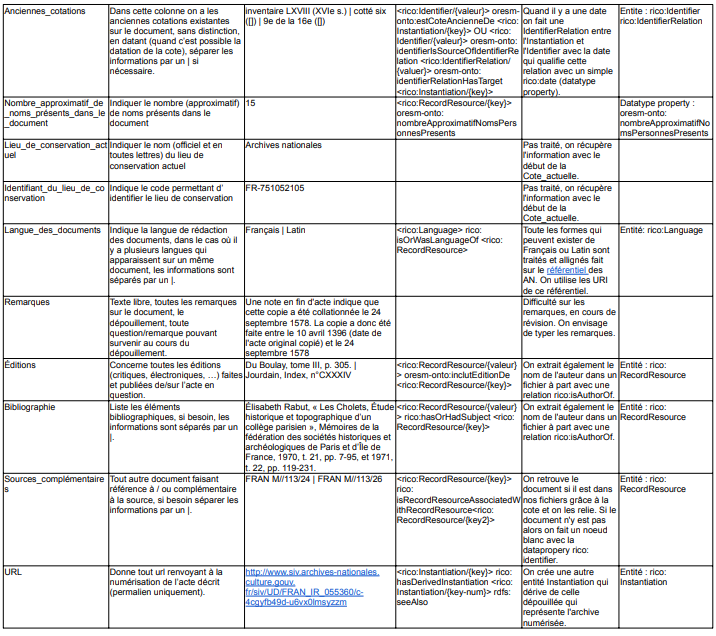
\includegraphics[width=1\linewidth]{annexes/mapping4.png}
\end{figure}

\chapter{Visualisation dans GraphDB Free}
\begin{figure}[!h]
    \centering
    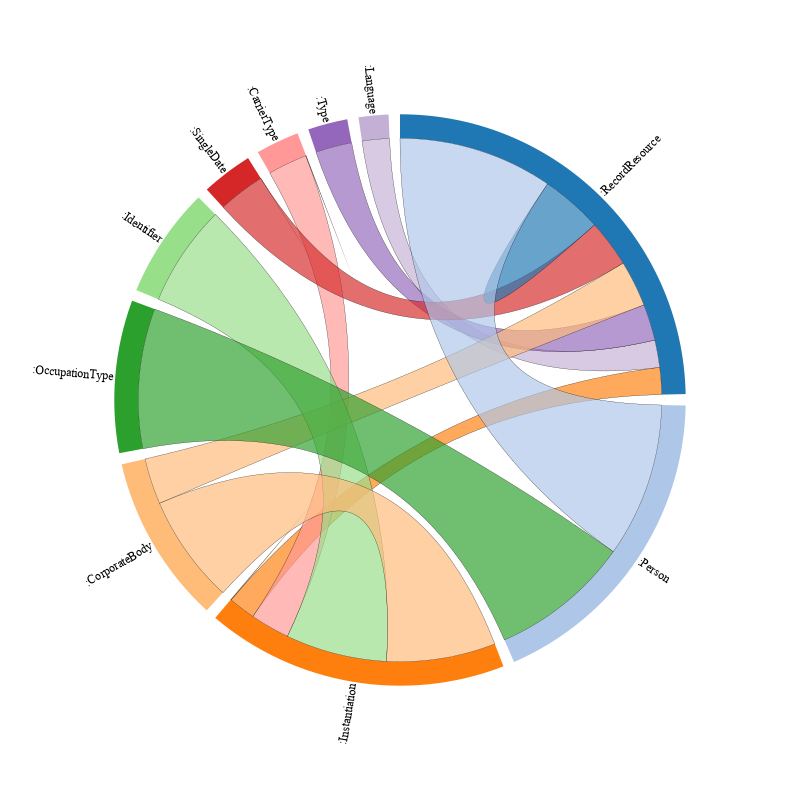
\includegraphics[width=0.8\linewidth]{annexes/dependencies-ORESM.png}
    \caption{Visualisation dans GraphDB Free qui représente la quantité de relations entre les différents types d'entités. \ref{chapitre6}}
    \label{fig:visualisation-classe-graphdb}
\end{figure}

\chapter{Requêtes SPARQL}
\label{sparql}
\begin{verbatim}
prefix oresm-onto: <http://data.oresm.fr/ontology#>
prefix rico: <https://www.ica.org/standards/RiC/ontology#>
prefix rdfs: <http://www.w3.org/2000/01/rdf-schema#>
prefix rdf: <http://www.w3.org/1999/02/22-rdf-syntax-ns#>
prefix xsd: <http://www.w3.org/2001/XMLSchema#>
PREFIX skos: <http://www.w3.org/2004/02/skos/core#>
PREFIX html: <http://www.w3.org/1999/xhtml>

#Récupère chaque rico:Person et les tris par nom de famille.

SELECT DISTINCT ?acteur ?prenom ?nomfamille (GROUP_CONCAT(DISTINCT 
?occupationl;separator='|') as ?occupations) (GROUP_CONCAT(?normalise;
separator = '\n') as ?toutes_dates) WHERE { 

    ?acteur rdf:type rico:Person.
    ?acteur rico:name ?nom.
    BIND(REPLACE(?nom,'.*([A-Z][a-àâçéèêëîïôûùüÿñæœ]+) ?(?:\\(|$|\\[).*','$1') 
    as ?nomfamille)
    BIND(REPLACE(?nom,'^(.+?) .+','$1') as ?prenom)
    
    OPTIONNAL{
    ?acteur rico:hasOrHadOccupationOfType ?occupation.
    ?occupation rdfs:label ?occupationl
    }
    
    ?record rico:isRelatedTo ?acteur; 
    rdfs:label ?nom_record ; 
    rdf:type ?record_ressource .
    ?record_ressource rdfs:subClassOf* rico:RecordResource.
   
    OPTIONNAL{
    ?record rico:isAssociatedWithDate ?date. 
    ?date rico:normalizedDateValue ?normalise
    }

}GROUP BY ?acteur ?prenom ?nomfamille ORDER BY ?nomfamille


---------------------------------------------------------

#Ajoute une relation rico:knows pour chaque personne qui est témoin du même acte. 


CONSTRUCT { ?personne1 rico:knows ?personne2 } WHERE { 
	?record oresm-onto:aPourTemoin ?personne1; 
            oresm-onto:aPourTemoin ?personne2.
    FILTER (?personne2 != ?personne1)
}


----------------------------------------------------------
#Compte le nombre de personne associé à une occupation.

SELECT (COUNT(?personne) as ?combien) ?occupationNom WHERE {
    ?personne rico:hasOrHadOccupationOfType ?occupation; rico:name ?noms.
    ?occupation rico:name ?occupationNom
} GROUP BY ?occupationNom

---------------------------------------------------------
\#Si le record a un testateur identifié alors c'est un testament


CONSTRUCT {
    ?testament 
    rico:isDocumentaryFormTypeOf 
    <http://data.oresm.fr/documentaryFormType/testament>
} WHERE { 
	?testateur oresm-onto:estTestateurDe ?testament.
}

---------------------------------------------------------
#Compte le nombre d'archives par langue et par siècle.

SELECT DISTINCT ?langueLabel ?siecle (COUNT(?record) as ?nombre) WHERE {
    ?record rico:hasOrHadLanguage ?langue; rico:isAssociatedWithDate ?date.
    ?langue skos:altLabel ?langueLabel.
    ?date rico:normalizedDateValue ?normalise.
    
    BIND(REPLACE(STR(YEAR(?normalise)+100),'[0-9]{2}$',' ème siècle') as ?siecle)
    
} GROUP BY ?langueLabel ?siecle ORDER BY ?siecle

---------------------------------------------------------
#Possible requête pour lier une femme ou une veuve à son mari
déjà présent dans le graphe identifié par le nom dans
le descriptive Note

PREFIX rico: <https://www.ica.org/standards/RiC/ontology#>
PREFIX rdf: <http://www.w3.org/1999/02/22-rdf-syntax-ns#>
PREFIX html: <http://www.w3.org/1999/xhtml>
CONSTRUCT {
    ?personne rico:hasOrHadSpouse ?acteur.
} where { 
    
	?personne a rico:Person ; 
        rico:descriptiveNote ?description; 
        rico:name ?nom_personne.
    ?acteur rdf:type rico:Agent; rico:name ?nom.
    BIND(REPLACE(str(?description),
    '[\\S\\s]+?(?=<html:p>)<html:p>([\\S\\s]+?) (\\[[^]]+\\])(?=<\\/html:p>)
    <\\/html:p>[\\S\\s]+','$1$2') as ?role).
    BIND(REPLACE(?role,"^[^A-Z]+(.*?)(?: et|,|\\[).*",'$1') as ?relatif).
    BIND(REPLACE(?role,"^([^A-Z]+).*?(?: et|,|\\[).*",'$1') as ?relation).
    
    FILTER(?relatif != '')
    FILTER(regex(?relatif,'[A-Z].*?[A-Z]'))
    FILTER(regex(?nom,?relatif))
    FILTER(regex(?relation,'femme|veuve'))
}
\end{verbatim}

\backmatter

\listoffigures
\tableofcontents
\end{document}
